%!TEX TS-program = xelatex
%!TEX encoding = UTF-8 Unicode

\documentclass[%10pt,
			   b5paper,
			   twoside
			   ]{book}

%\usepackage[cam,a3,center]{crop}

\usepackage{imakeidx}
\usepackage[T1]{fontenc}

\usepackage[top=1.23in,
			bottom=1.23in,
			left=.707in,
			right=1.23in
			%margin=1.23in,
		    %pass,
		    %showframe
		    ]{geometry}

\usepackage[parfill]{parskip} % Activate to begin paragraphs with an empty line rather than an indent
\usepackage{graphicx}
\usepackage{amssymb}
\usepackage{wrapfig}
\usepackage{float} % they need to be placed in specific locations with the [H] (e.g. \begin{table}[H])

\usepackage{paralist}
\usepackage{array}
\usepackage{longtable}
\usepackage{multirow}

\usepackage{url}
\usepackage[colorlinks]{hyperref}
\hypersetup{citecolor=black}
\hypersetup{linkcolor=black}
\hypersetup{urlcolor=black}
\usepackage{cleveref}

\usepackage{microtype} % Improves spacing
\usepackage{multicol}
\usepackage{pdfpages}

\usepackage{tikz}
\usetikzlibrary{shapes.geometric}
\usetikzlibrary{matrix}
\usetikzlibrary{snakes}

\usepackage{color}
\usepackage{lipsum}

\usepackage[framed,numbered]{sclang-prettifier}

% \makeindex[title=Indice dei nomi]

\graphicspath{{images/}}

%-------------------------------------------------------------
%------------------------------------------------ TIPOGRAFIA -
%-------------------------------------------------------------

\input{../_lib/fonts.tex}

\setlength{\columnsep}{.4in}


\setcounter{secnumdepth}{3}
\setcounter{tocdepth}{1}

%-------------------------------------------------------------
%---------------------------------------------------- HEADER -
%-------------------------------------------------------------

\usepackage{fancyhdr}

\fancypagestyle{plain}{%
\fancyhf{} % clear all header and footer fields
%\fancyhead[CO,CE]{---Draft---}
\fancyfoot[RO,LE]{\fontsize{18pt}{18pt}\selectfont\thepage} % except the center
\renewcommand{\headrulewidth}{0pt}
\renewcommand{\footrulewidth}{0pt}}
\pagestyle{plain}

%-------------------------------------------------------------
%----------------------------------------------------- TITLE -
%-------------------------------------------------------------

\makeatletter
%\frameattext{<backgroundcolor>}{linecolor}{<linewidth>}
\newdimen\extraxsep
\newdimen\extraysep
\extraxsep=20mm
\extraysep=20mm
\newcommand\frameattext[3]{%
  \linethickness{#3}%
  \AddToShipoutPicture*{%
    \AtTextLowerLeft{%text-boder
       \put(\LenToUnit{-,5\extraxsep},\LenToUnit{-0.5\extraysep}){\color{#1}%
             \rule{\dimexpr\textwidth+\extraxsep\relax}{\dimexpr\textheight+\extraysep\relax}}%
       \put(\LenToUnit{-,5\extraxsep},\LenToUnit{-0.5\extraysep}){\color{#2}%
       \framebox(\LenToUnit{\dimexpr\textwidth+\extraxsep\relax},%
                 \LenToUnit{\dimexpr\textheight+\extraysep\relax}){}
       }
    }%
  }%
}
%\frameatpage{<backgroundcolor>}{linecolor}{<linewidth>}
\newcommand\frameatpage[3]{%
  \linethickness{#3}%
  \AddToShipoutPicture*{%
    \AtPageLowerLeft{%page-border
      \put(0,0){\color{#1}\rule{\paperwidth}{\paperheight}}%
      \put(\LenToUnit{\@wholewidth},\LenToUnit{\@wholewidth}){%
       \color{#2}\framebox(\LenToUnit{\dimexpr\paperwidth-2\@wholewidth\relax},%
                  \LenToUnit{\dimexpr\paperheight-2\@wholewidth\relax}){}%
      }%
    }%
  }%
}

\makeatother

%-------------------------------------------------------------
%-------------------------------------------------- DOCUMENT -
%-------------------------------------------------------------

\begin{document}

\setlength{\columnsep}{.4in}

\frameattext{white}{black}{2pt}

\begin{center}
	~
	\vfill

    \fontsize{19}{19}\selectfont{Giuseppe SILVI}
    	\vspace{.3in}
		\noindent\makebox[\linewidth]{\rule{.3\paperwidth}{1pt}}
	\fontsize{51}{51}\selectfont{\emph{l'invito all'ascolto}} \\
		\vfill %\vspace{1in}
		~
		\vfill

    \fontsize{19}{19}\selectfont{COME/01 \\ esecuzione ed interpretazione della \\musica elettroacustica \\ 2016/2017} \\

		\vfill
	\fontsize{19}{19}\selectfont{draft 002\\ \today}

	\vfill
	~

\end{center}
%\maketitle

\thispagestyle{empty}

%\clearpage
%
%\thispagestyle{empty}
%
%~
%
%\clearpage
%
%\tableofcontents
%
%~\vfill
%
%
\includegraphics[width=.25\columnwidth]{images/by-nc-sa}\\
%\emph{A. Sax.} by Giuseppe Silvi is licensed under a Creative Commons \\
%Attribution-NonCommercial-ShareAlike 4.0 International License.\\
%Permissions beyond the scope of this license may be available at\\
%giuseppesilvi.com/asax.%\marginpar{prova}
%
%
\clearpage

%-------------------------------------------------------------
%-------------------------------------------------- COLOPHON -
%-------------------------------------------------------------

%!TEX TS-program = xelatex
%!TEX encoding = UTF-8 Unicode
% !TEX root = ../../2017-GS-COME01-INVITO-ASCOLTO.tex

%-------------------------------------------------------------
%-------------------------------------------------- COLOPHON -
%-------------------------------------------------------------

\thispagestyle{empty}

Conservatorio di Musica S. Cecilia di Roma \\
DIPARTIMENTO DI MUSICA ELETTRONICA \\
\emph{Esecuzione ed Interpretazione della Musica Elettronica - COME/01} \\
Triennio Accademico 2016-2019
\vfill

Attribution 4.0 International (CC BY 4.0)

You are free to:
\begin{description}
	\item[Share] - copy and redistribute the material in any medium or format
	\item[Adapt] - remix, transform, and build upon the material for any purpose, even commercially.
\end{description}

Under the following terms:
\begin{description}
	\item[Attribution] You must give appropriate credit, provide a link to the license, and indicate if
	changes were made. You may do so in any reasonable manner, but not in any way that suggests the licensor
	endorses you or your use.
	\item[No additional restrictions] You may not apply legal terms or technological measures that legally
	restrict others from doing anything the license permits.
\end{description}

Notices:\\
You do not have to comply with the license for elements of the material in the public domain or where your
use is permitted by an applicable exception or limitation. No warranties are given. The license may not give
you all of the permissions necessary for your intended use. For example, other rights such as publicity,
privacy, or moral rights may limit how you use the material.

\clearpage


\clearpage

%-------------------------------------------------------------
%---------------------------------------------------- INDICE -
%-------------------------------------------------------------

\tableofcontents
\thispagestyle{empty}

\clearpage

%-------------------------------------------------------------
%---------------------------------------------------- BIANCA -
%-------------------------------------------------------------

~
\thispagestyle{empty}

\clearpage

%-------------------------------------------------------------
%---------------------------------------------- INTRODUZIONE -
%-------------------------------------------------------------

%!TEX TS-program = xelatex
%!TEX encoding = UTF-8 Unicode
% !TEX root = ../../2017-GS-COME01-INVITO-ASCOLTO.tex

%-------------------------------------------------------------
%---------------------------------------------- INTRODUZIONE -
%-------------------------------------------------------------

\chapter*{Introduzione}
\addcontentsline{toc}{chapter}{Introduzione}

Operando la scelta dei brani per il corso di interpretazione ho provato a rispondere ad una domanda piuttosto semplice quanto necessaria: \emph{perché fare repertorio?} Questa domanda, prima di risposte, ha generato una successiva domanda: \emph{cos'è repertorio?} Ed anche rispondendo a queste prime domande ne è emersa una successiva: \emph{qual è il ruolo del repertorio nel fare contemporaneo?} Si ma \emph{cos'è contemporaneo?}.

Attraverso l'oscuro di questi dubbi ho individuato l'oscuro argomento del mio corso, quindi il focus sul repertorio: l'\emph{ascolto}. \emph{Fare repertorio nell'espressione del suo senso pi\`u completo \`e imparare ad ascoltare.}

Dato che le domande sono strettamente intrecciate tra loro, proverei a dare una prima definizione di uomo contemporaneo con le parole di Agamben\index{Agamben, Giorgio}:

\begin{quote}
	Contemporaneo è colui che riceve in pieno viso il fascio di tenebra che proviene dal suo tempo.
\end{quote}

È una definizione fortemente poetica che pone di nuovo la percezione al centro dell'asse uomo-tenebra. La contemporaneità è quindi un momento mobile del tempo che identifica la facoltà di osservare l'oscurità del tempo specifico.

L'osservazione può avvenire solo per distanza perché il contemporaneo, affinando la definizione con le parole di Nietzche, è intempestivo, inattuale.

\begin{quote}
	Appartiene veramente al suo tempo, è veramente contemporaneo colui che non coincide perfettamente con esso, non si adegua alle sue pretese ed è perciò, in questo senzo, inattuale; ma proprio per questo scarto e questo anacronismo, egli è capace pi\`u degli altri di percepire ed afferrare il suo tempo.
\end{quote}

La contemporaneità è quindi

\begin{quote}
	quella relazione col tempo che aderisce a esso attraverso una sfasatura e un anacronismo
\end{quote}

che ci permette di valutare, vedere ed analizzare, alla dovuta distanza. Spazio e tempo quindi legati nell'istante percettivo.

Il tempo del nostro repertorio

\begin{quote}
	è la contemporaneità, esso esige di essere contemporaneo dei testi e degli autori che esamina.
\end{quote}



Attraverso l'oscuro di questi dubbi ho individuato l'oscuro argomento del mio corso, quindi il repertorio, l'\emph{ascolto}: \emph{fare repertorio nell'espressione del suo senso pi\`u completo \`e imparare ad ascoltare.}

Crescere in un processo analitico-conoscitivo che amplifichi le capacità percettive, interpretando, nel significato pratico del termine, praticando. In questa direzione ho reso superfluo chiedersi \emph{perché fare repertorio} (per imparare ad ascoltare risponderemmo) ma al suo posto sorge spontaneamente la domanda \emph{come?} \emph{Come si fa repertorio?} Credo si possa fare repertorio solo ricostruendo, assemblando contesti sulle informazioni disponibili, affinch\'e la pratica poggi su una coscienza, ricostruita, che si stratifichi come pietra calcarea nel sapere sociale. Solo in questo senso il repertorio può essere, al pari della scrittura, esercizio, necessità, nutrimento della percezione.

\begin{quote}
	Alla scarsa attenzione alla problematica musicale da parte della riflessione estetica e filosofica in genere, fa riscontro - e alludo qui naturalmente in modo esclusivo alla situazione italiana - nei confronti della questione di una teoria generale della musica, disinteresse che non ha conseguenze solo su maggiori o minori profondità speculative, ma che ha generato una relativa arretratezza nel campo delle indagini pi\`u strettamente analitiche che esigono in via di principio opzioni di ordine teorico e metodico spesso apertamente confinanti nell'ambito delle questioni filosofiche [\ldots] La necessità di un punto di vista di una teoria generale si impone qui con particolare evidenza in stretta connessione con problematiche analitiche specifiche e con la consapevolezza del suo raggio di azione che raggiunge il problema della costruzione di un apparato categoriale capace di offrire strumenti per la comprensione delle strutture musicali di culture non europee, così come quello di un  rinnovamento della presentazione dei \emph{concetti fondamentali} che non può non avere conseguenze importanti nella didattica musicale. \footnote{Giovanni Piana (1991, p. 253, nota 14)}
\end{quote}

È un procedere che stratifica, solidifica conoscenza. Dopo aver studiato, letto ed interpretato \emph{Mantra} non si può tornare ad uno strato inferiore di coscienza, ad uno strato precedente di conoscenza. \emph{Mantra} si presenta come un paradigma del sapere musicale. Allo stesso tempo musicale, Cage, illumina la musica, sorride al senso del fare musica, porta l'idea di interprete ad un livello superiore, di manipolazione dell'idea, ai confini della libertà musicale e sociale, li dove spesso la mancata consapevolezza lascia smarriti e senza anima.


%-------------------------------------------------------------
%------------------------------- SUONO SEGNO INTERPRETAZIONE -
%-------------------------------------------------------------

%!TEX TS-program = xelatex
%!TEX encoding = UTF-8 Unicode
% !TEX root = ../../2017-GS-COME01-INVITO-ASCOLTO.tex

%-------------------------------------------------------------
%----------------------------- SUONO. SEGNO. INTERPRETAZIONE -
%-------------------------------------------------------------

\chapter*{Suono. Segno. Interpretazione.}
\addcontentsline{toc}{chapter}{Suono. Segno. Interpretazione.}

	\begin{flushright}
		\textit{Nella nostra anima c'\`e una incrinatura che, se sfiorata, \\
		risuona come un vaso prezioso riemerso dalle profondit\`a della terra} \\
		Wassilly Kandinsky - \emph{Lo Spirituale nell'Arte}
	\end{flushright}

	\begin{flushright}
		\textit{Music of Changes // John ChAnGEs} \\
		Pierre Boulez
	\end{flushright}

	\begin{flushright}
		\textit{Si dice che i compositori abbiano orecchio per la musica e \\
		di solito significa che non sentono nulla che arrivi alle loro orecchie. \\
		Le loro orecchie sono murate dai suoni di loro creazione.} \\
		John Cage - \emph{45' for a Speaker} (1954)
	\end{flushright}

\bigskip

%\begin{multicols}{2}

Le percezioni cambiano con il tempo. Ci sono diversi tempi, anche simultanei, del cambiamento.
Il tempo ciclico della riflessione. È quello breve, del pensiero ricorsivo, che non torna mai su se stesso identico al se stesso precedente.
In questo tempo la percezione stratifica, l'oggetto di senso percepito, osservato, muta, ne evolve il significato.
L'apparente movimento ciclico del pensiero ricorsivo non si muove ad anello, nbensì in una sorta di spirale per cui sì, bidimensionalmente, può apparire un ritornare, ma ad una visione almeno tridimensionale questo appare a forma di spirale.
Quadrimensionalmente questa è una spirale che si muove nel tempo, che quindi accupa uno spazio temporale ampio, del divenire. Due tempi quindi, quello ciclico, ricorsivo, e quello lungo, della mutazione nelle spazio-tempo.

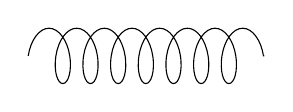
\begin{tikzpicture}[segment amplitude=10pt]
  \draw[snake=coil]                  (0,1) -- (3,1);
  %\draw[snake=coil,segment aspect=0] (0,0) -- (3,0);
\end{tikzpicture}

A queste percezioni che mutano nel tempo e nello spazio siamo abituati a dare nomi. Suono, è un nome.
L'idea di suono è separata dalla cosa che rappresenta.
Potremmo dire che il suo significato è rimasto quasi invariato nel corso dei tempi
In questo gli studi etimologici sono strumenti indispensabili.
Il rapporto sensoriale che identificheremo con le parole cambiano però piuttosto rapidamente.
Con la parola suono definiamo una percezione. Definiamo suono una percezione.
Il suo significato risale a epoche antiche.

Le arti del tempo condividono la stessa struttura percettiva: un testo fissato ed il suo alter ego evento momentaneo.

\begin{quote}
	la scrittura in tutti i campi si costituisce nel momento in cui si può disporre di un sistema di marcatori visivi che assolvono a fruizioni precedentemente affidate alla memoria o ad altri artifici più rudimentali\footnote{borio 9}
\end{quote}

Suono e Segno. I due stati dell'oggettivazione musicale sui quali l'interpretazione, sguardo ad oggettività limitata, vede collegamenti e potenzialità. Suono e gesto viaggiano su un asse temporale diverso da quello della sua rappresentazione. Ma circoscrivere il segno a “semplice” rappresentazione è grossolanamente sbagliato.

Se suono e gesto possiedono un tempo separato da quella della sua rappresentazione (tradizione orale) allora c'è da domandarsi cosa la scrittura abbia aggiunto e se si è verificata una eventuale perdita.

\begin{quote}
	il testo musicale [\ldots] solleva una pretesa normativa di fronte a chi lo legge\footnote{Borio}.
\end{quote}

Non ci vuole molto ad ipotizzare quindi una perdita di spontaneità e fantasia espressiva dell'interprete contemporaneo, incatenato alle regole scritte più del suo collega libero, che usava le parole piuttosto che i segni per imbrigliare il discorso musicale. Evidentemente quindi potrebbe risultare la perdita di spontanea immaginazione nel rapporto con il solo istinto musicale. Non si può nemmeno ignorare il fatto che è la forma scritta a regolare al tempo funzione informativa ed evolutiva tale da strutturare complesse relazioni orizzontali e verticali riconoscibili dalla memoria. Il segno che permette al raginamento di formare il tempo musicale. La scrittura come sistema di relazione tra segni nel tempo.

\begin{quote}
	la sua efficacia è strettamente connessa alla precisione e alla rapidità con cui vengono riconosciuti i simboli e i loro composti, cioè i tempi e modi con cui si svolge la lettura del testo\footnote{Borio}.
\end{quote}

L'evento momentaneo nella espressione della sua unicità è legato nel tempo stesso all'arte che rappresenta attraverso lo sguardo, la voce e il gesto dell'interprete. L'interpretazione nelle arti del tempo è manifestazione di una storia parallela a quella della percezione, della scrittura, e della pratica musicale. L'interpretazione è di fatto una riscrittura nel tempo del tempo. Ma ci deve essere una differenza tra l'interpretazione nel dominio orale piuttosto che scritto.

\begin{quote}
	lun discorso lineare e non ripetittivo per non parlare di una costruzione sillogistica, presuppine l'esistenza di un \emph{MEDIUM} che permetta alla psiche di sospendere le sue relazioni immediate; la scrittura è particolarmente adatta a tale scopo\footnote{Borio 14}.
\end{quote}

Nella composizione del percorso musicale quindi la pratica di scrittura è un mezzo per gestire limiti psico-cognitivi doiversi tra soggetti diversi. Non è quindi un paragone disumano tra oralità e scrittura quanto ognuno di questi in relazione all'uomo che li produce.

\begin{quote}
	alla base della scrittura moderna vi è dunque un processo di astrazione mediante cui il discorso temporale viene raffigurato nella successine spaziale\footnote{Borio 15}.
\end{quote}

Suono, evento momentaneo.

Segno, discorso temporale astratto.

Interpretazione, lettura multi-sensoriale del tempo. Solo l'interpretazione può riconoscere il progetto musicale celato nel testo e nella sua identità sonora.

\begin{center}
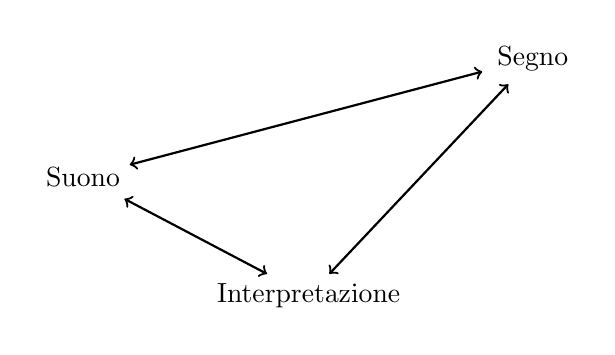
\begin{tikzpicture}[
    auto,
    arrow/.style = {
    	draw,
		thick,
		<->,
		shorten >=2pt
		}
  ]
\matrix [column sep=10mm, row sep=10mm] {
    & &	\node [] (segno) {Segno}; \\
	\node [] (suono) {Suono}; & &\\
    & \node [] (interpretazione) {Interpretazione}; &	 \\	
  };

\begin{scope} [every path/.style=arrow]
  	\path (suono) -- (segno);
	\path (interpretazione) -- (suono);
	\path (interpretazione) -- (segno);
\end{scope}
  
\end{tikzpicture}
\end{center}

\begin{quote}
	\ldots sono segni rivelatori delle cose, immagini delle parole, dotate di tal
	forza che, pur senza suono alcuno, ci trasmettono ciò che è stato detto da
	persone lontane: [le lettere, infatti, permettono alle parole di entrare in noi
	attraverso gli occhi e non attraverso l'udito]\footnote{controllare bene citazione isidoro di siviglia}
\end{quote}

questo vale quanto mai anche per la scrittura musicale, dove le “note” sono le immagini sonore dei suoni.


La musica, come le altre arti del tempo, danza, teatro, poesia presentano uno sdoppiamento su due piani dimensionali: testo ed evento.
La partitura musicale in particolare propone una dialettica tra testo e suoni che non si riscontra però in un copione o in notazioni coreografiche. Il testo stesso offre solo scansione metrica. Il testo musicale è prescrizione di un insieme di azioni e contemporaneamente è una prima oggettivazione di senso\footnote{Gianmario Borio, \emph{Segno e suono. Sulle funzioni della scrittura per la rappresentazione del pensiero musicale} in \emph{La scrittura come rappresentazione del pensiero musicale}. In nota Borio propone, per approfondimenti sull'esemplarità della notazione musicale nella relazione con una teoria generale dell'arte Nelson Goodman, \emph{I linguaggi dell'arte}}.

Queste considerazioni

%\end{multicols}

%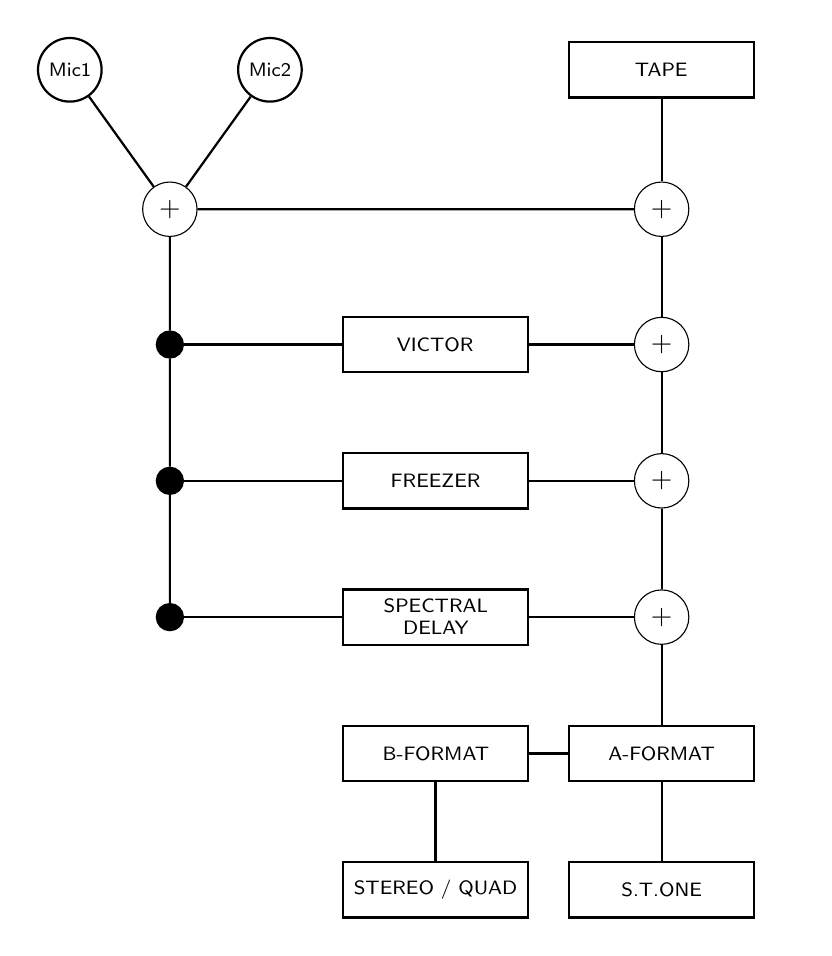
\begin{tikzpicture} [
    auto,
    mic/.style = {
    	font=\scriptsize\sffamily,
		circle,
		draw=black,
    	thick,
    	%fill=blue!20,
    	text width=2em,
    	text badly centered,
    	inner sep=1pt,
	},
    block/.style    = {
    	font=\scriptsize\sffamily,
    	rectangle,
		draw=black,
		thick,
		%fill=black!10,
		text width=6em,
		text centered,
		%rounded corners,
		minimum height=2em
		},
	line/.style = {
    	draw,
		thick,
		fill=black
		%shorten >=2pt
		},
	control/.style = {
    	draw,
		circle,
		thick,
		fill=black,
		%shorten >=2pt
		},
    arrow/.style = {
    	draw,
		thick,
		->,
		shorten >=2pt
		},
  ]
  % Define nodes in a matrix
  \matrix [column sep=5mm, row sep=10mm] {
	\node [mic] (mic1) {Mic1}; & \node [] (null1) {}; & \node [mic] (mic2) {Mic2}; & & \node [block] (tape) {TAPE}; & \\
	& \node [draw,circle] (inputs) {+}; & & & \node [draw,circle] (direct) {+}; & \\
	& \node [control] (node1) {}; & & \node [block] (victor) {VICTOR}; & \node [draw,circle] (mix1) {+}; & \\
	& \node [control] (node2) {}; & & \node [block] (freezer) {FREEZER}; & \node [draw,circle] (mix2) {+}; & \\
	& \node [control] (node3) {}; & & \node [block] (sdelay) {SPECTRAL DELAY}; & \node [draw,circle] (mix3) {+}; & \\
	& & & \node [block] (bfmt) {B-FORMAT}; & \node [block] (afmt) {A-FORMAT}; & \\
	& & & \node [block] (outputs) {STEREO / QUAD}; & \node [block] (stone) {S.T.ONE}; & \\
  };

  \begin{scope} [every path/.style=line]
  	\path (mic1) -- (inputs) -- (node1) -- (node2) -- (node3);
	\path (mic2) -- (inputs) -- (direct);
    \path (node1) -- (victor) -- (mix1);
    \path (node2) -- (freezer) -- (mix2);
    \path (node3) -- (sdelay) -- (mix3);
    \path (tape) -- (direct) -- (mix1) -- (mix2) -- (mix3);
    \path (mix3) -- (afmt) -- (stone);
    \path (afmt) -- (bfmt) -- (outputs);

  \end{scope}

\end{tikzpicture}



%-------------------------------------------------------------
%------------------------------------ IMAGINARY LANDSCAPE N3 -
%-------------------------------------------------------------

%!TEX TS-program = xelatex
%!TEX encoding = UTF-8 Unicode
% !TEX root = ../../2017-GS-COME01-INVITO-ASCOLTO.tex

\clearpage

\thispagestyle{empty}

\includepdf[scale=1.05,
		    pagecommand={
		    	\begin{tikzpicture}[
					remember picture,
					overlay]
		    	\node [xshift=2cm,yshift=1cm] at (current page.south west) {\color{white}{\emph{Roberto \textbf{Masotti}}}};
				\end{tikzpicture}}
		    ]{images/masotti/cage.pdf}

\clearpage

%-------------------------------------------------------------
%------------------------- JOHN CAGE - IMAGINARY LANDSCAPE 3 -
%-------------------------------------------------------------

\chapter*{1942. John Cage. \\ \emph{Imaginary Landscape n. 3}.}
\addcontentsline{toc}{chapter}{1942. John Cage. \emph{Imaginary Landscape n. 3}.}

%	\begin{flushright}
%		\textit{Nella nostra anima c'\`e una incrinatura che, se sfiorata, \\
%		risuona come un vaso prezioso riemerso dalle profondit\`a della terra} \\
%		Wassilly Kandinsky - \emph{Lo Spirituale nell'Arte}
%	\end{flushright}
%
%	\begin{flushright}
%		\textit{Music of Changes // John ChAnGEs} \\
%		Pierre Boulez
%	\end{flushright}
%
%	\begin{flushright}
%		\textit{Si dice che i compositori abbiano orecchio per la musica e \\
%		di solito significa che non sentono nulla che arrivi alle loro orecchie. \\
%		Le loro orecchie sono murate dai suoni di loro creazione.} \\
%		John Cage - \emph{45' for a Speaker} (1954)
%	\end{flushright}
%
%\bigskip

\begin{lstlisting}[style=SuperCollider-IDE]
// Constant Frequency Record
(
SynthDef("constant-frequency", { arg out=0;
    Out.ar(out,
    SinOsc.ar(1000,0, 0.2))
}).play;
s.record(duration:900, numChannels:0);
)

// Continuously Variable Frequency Record
(
SynthDef("continuously-variable-frequency", { arg out=0;
    Out.ar(out,
    SinOsc.ar(LFNoise2.ar(0.5).range(400, 4000), 0, 0.2))
}).play;
s.record(duration:900, numChannels:0);
)

// Generator Whine Record
(
SynthDef("generator-whine", { arg out=0;
    Out.ar(out,
        LFBrownNoise2.ar(2000, 1, 0, 0.25) + SinOsc.ar(LFNoise2.ar(1234).range(9751, 10000),0, 0.012345)
    )
}).play;
s.record(duration:900);
)
\end{lstlisting}


%-------------------------------------------------------------
%------------------------------------------------- STUDIE II -
%-------------------------------------------------------------

%!TEX TS-program = xelatex
%!TEX encoding = UTF-8 Unicode
% !TEX root = ../../2017-GS-COME01-INVITO-ASCOLTO.tex

\clearpage

\thispagestyle{empty}

\includepdf[scale=1.03,
		    pagecommand={
		    	\begin{tikzpicture}[
					remember picture,
					overlay]
		    	\node [xshift=2cm,yshift=1cm] at (current page.south west) {\color{white}{\emph{Heinz \textbf{Karnine}}}};
				\end{tikzpicture}}
		    ]{images/stockhausen/stockhausen.pdf}

\clearpage

%-------------------------------------------------------------
%--------------------------- KARLHEINZ STOCKHAUSEN STUDIE II -
%-------------------------------------------------------------

\chapter*{1956.\\ Karlheinz STOCKHAUSEN. \\ \emph{Studie II}.}
\addcontentsline{toc}{chapter}{1956. Karlheinz STOCKHAUSEN. \emph{Studie II}.}

\vfill

Lo \emph{StudieII} nel repertorio elettroacustico rappresenta il reperto archeologico, il grado zero della conoscenza elettronica, pensiero cristallizzato ed articolato in testo musicale tuttora leggibile, interpretabile, attraverso un processo compositivo ri-eseguibile.

Il materiale sonoro è quanto di più antico in termini di produzione umana elettronica in musica. Per ricostruire lo spazio tecnico di lavoro che ha plasmato quelle idee musicali, le possibilità tecniche ed il lessico specifico ci serviamo delle parole di alcuni personaggi di quella storia. Così Prieberg scrive dei suoni sinusoidali in \emph{Musica Ex Machina}:

\begin{quote}
	[\ldots] Il suono sinusoidale è un fenomeno completamente nuovo nella musica. Si intende un suono senza armonici, cioè il suono nudo, che forma una vibrazione sinusoidale. È un prodotto dei vibratori graduati elettronici, con i quali di solito vengono prodotti nelle stazioni radio il segnale orario, il diapason per i musicisti e – prima e dopo l’orario giornaliero di trasmissione – le frequenze pilota.
	[\ldots] è veramente senza luogo, una vibrazione isolata, che nasce ed è amplificata nella valvola elettronica e diventa udibile solo nell’altoparlante. Il suono sinusoidale si sottrae a ogni definizione all’infuori di quella con il numero di \emph{Hertz} delle sue vibrazioni. Girando l’interruttore del condensatore del generatore elettronico lo si può spostare in qualsiasi punto dell’intera sfera uditiva\footcite[pag. 170--179]{prieberg:mexm}.
\end{quote}

Lo stesso Prieberg si serve poi delle parole di Herbert Eimert\footnote{
	Herbert Eimert, tra le due guerre lavorava alla Radio di Colonia dal 1927 al 1933. Nel 1945, sotto l'amministrazione britannica, fu il primo tecnico assunto dalla nuova Radio di Colonia (\emph{NWDR}). Nel 1951 insieme a Werner Meyer-Eppler persuade Hanns Hartmann, direttore di NWDR, a creare il primo studio per la musica elettronica che diresse fino al 1962, quando gli successe Karlheinz Stockhausen. Insieme a Hans Ulrich Humpert, scrisse il \emph{Lexikon der elektronischen Musik}, (dizionario della musica elettronica).
} il quale descrive il suono sinusoidale come

\begin{quote}
  neutrale e già abbastanza forte a un’intensità media, perciò non è affatto smorto e insussistente. Siccome manca degli armonici caratteristici, non ha alcun timbro ben definito. Il suo contrassegno principale è la diretta immediatezza del suono. Dipende dalla sua natura elettrica il fatto che esso risuona come una corrente uniforme, rigido e non modulato\footcite[\emph{idem}]{prieberg:mexm}.
\end{quote}

Prieberg descrive alcune pratiche e tecniche di laboratorio di quegli anni

\begin{quote}
	[\ldots] Suoni sinusoidali possono essere sovrapposti in qualsiasi numero e frequenza, sia armonicamente, di modo che si ottiene un suono con un corteggio di armonici naturale, sia non armonicamente, di modo che nasce una cosiddetta « mescolanza di suoni ». [\ldots] L’inizio del suono coincide con l’innesto, e con il disinnesto s’interrompe immediatamente. Perciò il carattere del suono deve essere aggiunto alla composizione e per fare questo si offrono le più varie possibilità. Con le forbici il compositore taglia via dal nastro inciso non solo la lunghezza ma anche le cosiddette « curve di inviluppo », le caratteristiche forme dei suoi elementi acustici. [. . . ] Inoltre egli può servirsi di un apparecchio di risonanza o della riverberazione che si trova in ogni stazione radio. Se la formazione lo soddisfa, inizia allora il montaggio dei molti piccoli ritagli di nastro nella disposizione ritmica desiderata.
	Complicatissimi passaggi dinamici nascono sotto un costante controllo con il centimetro. Siccome il compositore conosce la velocità del nastro, di solito $ 76,2 $ o $ 38,1 $ centimetri al secondo, misurando la lunghezza di pause e suoni egli può produrre ritmi « irrazionali » precisissimi, mentre ogni compositore di musica strumentale fallirebbe senza speranza in quest’impresa.
\end{quote}

Su Studio 2

\begin{quote}
	[\ldots] Esistono diverse possibilità di fissare la musica elettronica in qualcosa di simile a uno « spartito ». Una « partitura » elettronica, lo Studio II di Karlheinz Stockhausen, è già stampata. Un progetto di costruzione, un disegno tecnico per cosìdire, documento unico di una musica dell’avvenire. Al primo sguardo si presenta come un disegno affascinante di vari rettangoli e triangoli.
	L’idea della notazione, cioè la distribuzione del tempo in senso orizzontale da sinistra a destra, e la collocazione delle note e dei suoni in senso verticale, dal basso in alto, rimane inalterata. Invece è nuova l’annotazione assoluta. Le note musicali si limitano a dare un sistema di riferimento. Esse sono relative. Il loro valore assoluto dipende da una convenzione non obbligatoria, dall’altezza relativa del diapason. Un’esecuzione più o meno autentica – anche per quel che riguarda l’altezza di suono – riesce unicamente se si ha una precisa conoscenza di questa convenzione. Invece la musica elettronica è incisa su nastro conformemente alle idee del compositore. L’interpretazione non è nénecessaria népossibile. Perciò la rappresentazione grafica dell’opera elettronica deve essere vera e assolutamente precisa: il tecnico dello studio lavora su di essa. Molte novità saltano agli occhi. L’altezza del suono si misura in Hertz, cioè in vibrazioni al secondo; l’intensità si esprime in Decibel, cioè nei gradi di un aumento del 26 per cento circa dell’energia sonora, che vengono ancora percepiti dall’orecchio – non più con indicazioni così vaghe come forte e pianissimo; per la velocità si evitano le arbitrarie indicazioni andante, presto o largo, si calcola secondo i centimetri del nastro che scorre. Al posto dell’approssimazione interpretativa è subentrata matematica esattezza. La « partitura » elettronica di Stockhausen corrisponde alle premesse di un caso compositivo speciale: le centonovantatre mescolanze di suoni, di cinque suoni sinusoidali ciascuno, che egli usa, non sono montati singolarmente ma risultano dalla relazione meccanica dei suoni sinusoidali sonati uno dopo l’altro nella riverberazione. Siccome si tratta esclusivamente di suoni di uguale intensità e con intervalli costanti, ne consegue subito che una simile annotazione semplificata può valere soltanto per questa composizione elettronica.

	Se si esamina ora nei particolari, si vede che la parte superiore della « partitura » – un po’ più della metà – è costituita da un sistema di linee che comprende lo spazio da 100 fino a $ 17200 $ \emph{Hertz} sfruttato da Stockhausen nello Studio II. Rettangoli di varie forme simbolizzano blocchi di cinque suoni sinusoidali ciascuno, cioè mescolanze di suoni. Sotto questa parte la lunghezza dei blocchi è riportata ancora una volta su di una scala in centimetri di nastro. $ 76,2 $ centimetri corrispondono alla velocità allora usuale del nastro. Più sotto ancora vi è un secondo più sottile sistema di linee per la dinamica da 402 fino a 0 decibel. L’altezza del grafico in questo sistema indica l’intensità corrispondente. Le sue forme determinano i contorni, cioè le curve di inviluppo delle mescolanze dei suoni. In alcuni punti dei due sistemi mancano figure, il che significa pausa. Anche la durata è visibile dal numero nella scala delle lunghezze. Una pagina della partitura rappresenta all’incirca sei secondi di musica.
	I primi sette pezzi elettronici dello studio di Colonia [\ldots] Sono come uno scenario acustico, che provoca senza dubbio eccitamenti molto violenti i quali, pur non causando uno shock, opprimono tuttavia in modo quasi insopportabile il sistema nervoso.
\end{quote}

da La Musica Elettronica3

\begin{quote}
	[\ldots] L’articolazione e l’esatto metodo di produzione del materiale sono stati interamente esposti nella prefazione alla “partitura”, una delle rare rappresentazioni di musica elettronica pubblicate: si potrà rimandare ad essa. In effetti, in essa si ottiene una fusione molto maggiore degli “elementi” all’interno dei “suoni complessi”. Essa è dovuta, in primo luogo, alla loro “uguaglianza dinamica” ed alla complessità molto più grande dei loro rapporti armonici (ricordiamo che nel Primo Studio non si trattava di spettri “armonici” propriamente detti, centrati su un fondamentale unico; almeno tutti gli intervalli facenti parte di un blocco erano degli intervalli giusti, degli intervalli semplici e “trasparenti”). Essa è anche dovuta, per alcuni di essi (per i più “agglomeranti”), al serrarsi di questi intervalli costitutivi che provoca (non soltanto per la percezione, ma, si potrebbe dire, oggettivamente) la distruzione reciproca delle periodicità individuali e (come già il cromatismo simultaneo nelle musiche strumentali di cui abbiamo parlato nel primo capitolo) genera dei veri rumori (molto controllati, tuttavia). Inoltre, l’utilizzazione della camera a eco (“naturale”) come uno degli stessi mezzi della produzione sonora (metodo che reintroduce fin da allora un elemento non elettronico e per questo non strettamente controllato) rinforza ancora la fusione delle componenti (valorizzando i legami interferenziali) e conferisce ai risultati un’unità supplementare, dovuta al colore proprio di cui riveste in un certo senso tutto ciò che passa attraverso di essa.

	Infine, l’attacco simultaneo di diversi blocchi di questa specie da cui si ritagliano eventualmente le regioni armoniche (e la cui ulteriore evoluzione divergente dà, per contrasto, conferma), ed il fatto che Stockhausen abbia superato su questi attacchi di un poco le soglie di registrazione del nastro magnetico (di passare nella zona “rossa” dei potenziometri: fino a + 6dB), producendo, con la distorsione che ne deriva, dei veri transitori, paragonabili agli attacchi di certi strumenti (a percussione), contribuiva ad ottenere dei fenomeni sonori molto più unitari, la cui unità era già caratterizzata da un certo tasso di evoluzione interna, e li rendeva capaci di sopportare meglio il paragone con il carattere “organico” dei fenomeni naturali. Certo, a questo si univa una (molto relativa, ma innegabile nel rigore della prospettiva iniziale) perdita di controllo. Tuttavia le immediate conclusioni che se ne sarebbero potute tirare, le conseguenze che questo avrebbe avuto, nel senso di un certo ammorbidimento dei principi di realizzazione (e in primo luogo di concezione) non erano il solo insegnamento che se ne potesse trarre: Stockhausen (e coloro che seguivano da vicino le sue esperienze cominciando eventualmente a dedicarsi ad esperienze parallele) aveva appreso qui ogni sorta di nozioni precise sulla struttura dei fatti sonori, sulla possibilità di continuare a ricercarne il controllo integrale, anche se questo dovesse durare per un periodo abbastanza lungo e passare attraverso tappe apparentemente in contraddizione.
	In effetti, fin dal compimento del Primo Studio di Stockhausen, altri compositori erano stati invitati a lavorare temporeneemente allo studio di Colonia ed a realizzarvi una composizione per forza di cose modesta. Cosi, alla fine del 1954, una prima esecuzione dei lavori (che occupavano la metà di un concerto) potévenir proposta al pubblico (l’altra parte comprendeva esecuzioni di nuova musica americana da parte di John Cage e di David Tudor). Ad eccezione di qualche dettaglio, tuttavia, nessuno di questi lavori apportava nulla di fondamentalmente nuovo rispetto alle realizzazioni di Stockhausen.

	[\ldots] fenomeni paragonabili fino a un certo punto agli aggregati più indivisibili del Secondo Studio di Stockhausen, potevano essere ottenuti filtrando un fenomeno elettronico il meno periodico, il più disordinato possibile, la cui applicazione acustica si chiama “rumore bianco”. Ed infine alcuni momenti dell’una o dell’altra composizione particolarmente movimentati, particolarmente “microstrutturati” provavano (soprattutto se accelerati ancora, cosa di cui si poteva fare esperienza quotidiana durante il lavoro di studio) che si potevano raggiungere unità di una nuova specie, la cui instabilità, la cui mobilità, sarebbe una delle caratteristiche principali, che le contrapporrebbe dunque in maniera molto netta alla maggior parte dei suoni strumentali (analoghe solo alle misture a un tempo molto dense e molto rapide, come ne esistevano già, per esempio nella seconda delle prime Structures per due pianoforti di Boulez, o nei Kontrapunkte di Stockhausen). Prescindendo dalla perdita di controllo che il tentativo di sistematizzare dei fenomeni di questo tipo poteva rappresentare (e che potrebbe, per lo meno provvisoriamente, essere compensato da criteri di determinazione statistica) era proprio questo l’effetto di una di quelle “immaginazioni concrete” di cui dicevamo, che furono all’origine della nascita della musica seriale generalizzata, immaginazione che ci sforziamo dunque, intravedendola, di rendere attuale con un massimo di efficacia, ad un tempo “espressiva” (cioè piuttosto “qualitativa”) e strutturale (o più “quantitativa”). Sembrava che ci fossero delle vie per condurre a questo senza passare per il missaggio ed il montaggio di elementi sinusoidali (operazione naturalmente fastidiosa nel caso in cui si vogliano realizzare dei fenomeni formalmente antinomici rispetto alla sinusoide – e del resto poco efficaci a causa dei “rumori di fondo,” nel senso molto generale della parola, che la molteplicità delle operazioni introduce ed accumula). Le sinusoidi non rappresentarono dunque più che uno degli estremi di un campo di cui gli altri due “poli” simbolici sembrano essere: l’onda periodica “angolare” cioè il meno sinusoidale possibile, definibile in termini di “impulso” (dente di sega, “ago” o rettangolo) ed il “rumore bianco” o processo vibratorio il meno periodico possibile. Questo allargamento delte “riserve” materiali a cui poteva attingere il compositore apriva ad un tratto alla musica elettronica uno spazio figurativo molto pid ricco, molto più duttile. Se i compositori sapessero rivelarsi sufficientemente attenti, la luce momentanea (ed in alcuni casi del tutto relativa) del principio del controllo integrale, potrebbe non essere che una specie di astuzia per permettere l’appropriazione e la progressiva realizzazione di questi materiali sonori in diverse tappe. Tuttavia la prima di esse sarebbe una tappa in cui l’accento sarebbe posto più sovente, perlomeno per una parte dei compositori (e non necessariamente per i meno “prospettici”), sull’aspetto qualitativo, spontaneo, e quindi sulla generazione relativamente empirica, talvolta davvero improvvisata, delle nuove sonorità).
	[\ldots]
\end{quote}

da Musica Espansa4

\begin{quote}
	Gran parte dell’esperienza seriale elettronica maturata a Colonia è sorretta dall’operare teorico a compositivo di Stockhausen, dalla sua estrema fiducia nell’analisi cognitiva e da una metodologia scientifica di lavoro. Nel periodo dal 1953 al 1954, egli realizza alla WDR i pezzi elettronici Studie I e II, che rimangono tra i progetti musicali più rappresentativi di quella stagione musicale. Un condensato di riflessione teorica e di tecnica realizzativa, ma anche di scontro compositivo con il materiale e con i problemi della percezione musicale\footnote{(nota presente nel testo originale) Lo Studie II è inoltre il primo esempio di musica elettronica rappresentata da una partitura, un tentativo riuscito di creare una mediazione tra gesto formale e ascolto, mediante una descrizione grafica puntuale dello spazio sonoro: ampiezze, durate, misture frequenziali, inviluppi, densità verticale e movimento delle sequenze nel tempo. Dal punto di vista della grafia musicale nella musica elettronica degli anni Cinquanta, esistono altri esempi importanti, tra cui Incontri di fasce sonore (1956) di F. Evangelisti, e Artikulation (1958) di G. Ligeti. Entrambe hanno avuto una stesura che si avvicina a delle partiture di ascolto. Altre musiche concrete o elettroniche dispongono di partiture che vanno intese come partiture di lavoro, tra queste: Timbre-Durèes (1952) di O. Messiaen, Essay (1957) di M. Koenig. Il problema di una grafia della musica elettronica è anche contraddittorio per il significato stesso di partitura, cioè di mezzo simbolico non astratto ma finalizzato per l’esecuzione musicale. Il nastro magnetico è di per séla partitura.}

	Se lo Studie I può essere considerato una prova generale importante di progettazione musicale nel laboratorio della serialità elettronica, lo Studie II rivela un approfondimento compositivo indirizzato a ricercare una maggiore caratterizzazione interna dei materiali elettronici, a un maggiore contrasto tra le diverse tipologie delle misture sonore. In particolare, caratterizzando il pezzo con un uso delle strutture frequenziali molto più ricco e complesso, caricato da una bassa armonicità, in cui prevale alla fine una risultante timbrica assimilabile a quella ottenuta con rumori variamente filtrati e inviluppati. La contrapposizione tra i diversi transitori di attacco e tra le dinamiche è molto più netta; il fortissimo si avvale anche di una controllata saturazione dinamica del magnetofono, che conferisce di conseguenza una maggiore “coloratura” che, come sottolinea Henri Pousseur, “ contribuiva a ottenere dei fenomeni sonori molto più unitari, la cui unità era già caratterizzata da un certo tasso di evoluzione interna, che li rendeva capaci di sopportare meglio il paragone con il carattere organico dei fenomeni naturali”6.
	è utile portare l’attenzione sulla definizione di “organico” in contrapposizione al non organico che Pousseur utilizza nella descrizione del modo di suonare di certi blocchi sonori dello Studie II. Tale osservazione mette in luce uno degli aspetti di maggiore criticità della musica elettronica seriale, dovuta all’immobilità interna del suono. alla mancanza di microarticolazione della materia che conferisce viceversa una stimolazione percettiva e un interesse nell’ascolto e che ci permette di parlare di timbro e di agglomerati sinusoidali, cosa che Stockhausen aveva rilevato.
	Da un lato, il permutare e il combinare continuo dei parametri acustici delle “misture sonore” non facilita l’articolazione del tessuto sonoro, a causa del prodursi di una continua indifferenziazione, dovuta anche all’esiguo numero di parziali che compongono in genere le misture; dall’altra le difficoltà intrinseche nella realizzazione di una vera e propria sintesi additiva del timbro. Quindi il “comporre il suono” con i mezzi tecnologici dell’epoca, conduce ad accentuare volutamente soluzioni più dirette. Da qui l’introduzione di accorgimenti elaborativi estranei, come il passaggio delle misture nella “camera di riverberazione”, con lo scopo di conferire al risultato contorni “di disturbo” non prevedibili e quindi aleatori, in grado di dare respiro e circolazione sanguigna ai blocchi di suono.
	[...] In generale l’ascolto delle opere realizzate nello Studio di Colonia rivela una difficoltà nell’uscire da un’omologazione timbrica e da una economia dei materiali che non permette di ottenere una maggiore flessibilità linguistica.
	è individuabile un interesse primario rivolto soprattutto al sistema delle frequenze, che guida il procedere compositivo anche in un simile contesto sperimentale; Stockhausen, per esempio, utilizza in Studie II un rapporto di 5:1 suddiviso in 25 parti. Probabilmente ha ragione Franco Evangelisti quando sottolinea la necessità di ricorrere a rapporti di distanza, nello spazio frequenziale, espressi da numeri non interi, come condizione per uscire da certi vincoli di periodicità nella generazione spettrale dei suoni e conquistare realmente un diverso mondo sonoro. La sua composizione Incontri di fasce sonore (1956) è l’ultimissimo esempio di una musica elettronica che parte da un’idea costruttiva del timbro secondo il modello delle misture sonore sinusoidali, anche se esistono nel pezzo altre soluzioni a sostegno di una maggiore ricchezza di materiale disponibile. Scrive Evangelisti a proposito dell’organizzazione delle misture sonore presenti nella sua opera:

	\begin{quote}
		La suddivisione dello spazio sonoro e delle sue durate è stata concepita in base ai rapporti psicofisici e in funzione dei parametri degli stessi. La scala delle grequenze è stata suddivisa in 91 gradi a partire dalla frequenza più bassa di 87 Hz alla più alta di 11 ̇950 Hz. Il problema fondamentale è stato qello di non stabilire rapporti di armonia di nessun genere, espressi mediante numeri razionali interi, come per esempio nella scala temperata il rapporto di 2:1, o come nello studio di k. Stockhausen il rapporto di 5:1. [...]
	\end{quote}

La questione non risolta della mobilità interna del suono e della diversificazione dei materiali è un problema di tale complessità che gli assiomi iniziali vengono ben presto rivisitati e frantumata così l’estetica dell’elettronica pura.

\end{quote}


%-------------------------------------------------------------
%------------------------------------------- CARTRIDGE MUSIC -
%-------------------------------------------------------------

%!TEX TS-program = xelatex
%!TEX encoding = UTF-8 Unicode
% !TEX root = ../../2017-GS-COME01-INVITO-ASCOLTO.tex

\clearpage

\thispagestyle{empty}

\includepdf[scale=1.05,
		    pagecommand={
		    	\begin{tikzpicture}[
					remember picture,
					overlay]
		    	\node [xshift=2cm,yshift=1cm] at (current page.south west) {\color{white}{\emph{Roberto \textbf{Masotti}}}};
				\end{tikzpicture}}
		    ]{images/masotti/cage.pdf}

\clearpage

%-------------------------------------------------------------
%------------------------------- JOHN CAGE - CARTRIDGE MUSIC -
%-------------------------------------------------------------

\chapter*{1960. John Cage. \\ \emph{Cartridge Music}.}
\addcontentsline{toc}{chapter}{1960. John Cage. \emph{Cartridge Music}.}

	\begin{flushright}
		\textit{Nella nostra anima c'\`e una incrinatura che, se sfiorata, \\
		risuona come un vaso prezioso riemerso dalle profondit\`a della terra} \\
		Wassilly Kandinsky - \emph{Lo Spirituale nell'Arte}
	\end{flushright}

	\begin{flushright}
		\textit{Music of Changes // John ChAnGEs} \\
		Pierre Boulez
	\end{flushright}

	\begin{flushright}
		\textit{Si dice che i compositori abbiano orecchio per la musica e \\
		di solito significa che non sentono nulla che arrivi alle loro orecchie. \\
		Le loro orecchie sono murate dai suoni di loro creazione.} \\
		John Cage - \emph{45' for a Speaker} (1954)
	\end{flushright}

\bigskip

\begin{multicols}{2}

\begin{quote}
	Ogni opera d'arte \`e figlia del suo tempo, e spesso \`e madre dei nostri
	sentimenti.

	Analogamente, ogni periodo culturale esprime una sua arte, che non si ripeter\`a mai pi\`u.
	Lo stesso sforzo di ridar vita a principi estetici del passato pu\`o creare al massimo delle opere d'arte che sembrano bambini nati morti.
	Noi non possiamo, ad esempio, avere la sensibilit\`a e la vita interiore\footnote{Wassilly Kandinsky, \emph{Lo Spirituale nell'Arte}, SE. 1989}\ldots
\end{quote}

di John Cage, in luogo degli antichi Greci, come avrebbe continuato Kandinsky.
Ci deve essere un certo grado di consapevolezza in relazione al livello di
comprensione-incomprensione del pensiero di John Cage. Ma ammettendo di
averlo compreso, per quanto noi potremmo approfondire lo studio del suo
pensiero e della sua musica, potremmo solo arrivare ad imitarne alcuni tratti
stilistici. E se tentassimo di

\begin{quote}
	adottare i loro princ\`{\i}pi, non faremmo che produrre forme simili alle loro, ma prive di anima\footnote{\emph{idem}}.
\end{quote}

Questo non esclude che si possa riuscire ad entrare in contatto con le
motivazioni e gli stimoli artistici, soprattutto
e si attinge ai tratti
condivisi tra le somiglianze delle forme artistiche,

\begin{quote}
	delle aspirazioni interiori e degli ideali (che un tempo erano stati raggiunti
	e poi vennero dimenticati), la somiglianza cio\`e fra i climi culturali di due
	epoche che pu\`o portare alla ripresa di forme che erano gi\`a state utilizzate in
	passato per esprimere le stesse tensioni\footnote{\emph{idem}}.
\end{quote}

Costruire il repertorio, utilizzare il tempo presente per reinventare il tempo passato.
Respirare la stessa aria di un autore non pi\`u presente attraverso la comprensione, intima,
a livello percettivo, delle molteplici ineffabilit\`a della sua epoca.
Consumare la sua poetica acquisendo ogni io sotteso e nascosto. Percepirne il dopo,
il passato meno passato delle conseguenze lasciate al mondo, al suo futuro.
Tutto questo, di un personaggio poliforme ed enorme come John Cage, \`e piuttosto complesso.

%John Cage \`e stato al mondo in maniera totale.

Essere John Cage, \emph{compositore}: ha scritto testi, libri, ha tenuto conferenze, ha dipinto,
ha consultato gli oracoli, ha meditato, ha suonato, ha indagato, ha scritto musica.

%Questo essere, di una sensibilit\`a totale, significa utilizzare la percezione attraverso tutti i canali percettivi di cui si \`e dotati.

In questo senso l'attivit\`a artistica, plastica, sonora, letteraria \`e manifestazione di uno
stesso percepire comune.

Nel luogo temporale di John Cage c'\`e la grande depressione statunitense che trova al suo rientro dall'Europa,
con la quale deve fare i conti, per la prima volta, per guadagnarsi da vivere. Lo fa a suo modo,
sulle tracce di quello che negli anni settanta definir\`a anarchia:

\begin{quote}
	I'm an anarchist. I don't know whether the adjective is pure and simple, or philosophical, or what, but I don't
	like government! And I don't like institutions! And I don't have any confidence in even good institutions.\footnote{John
		Cage at Seventy: An Interview by Stephen Montague. American Music, Summer 1985. Ubu.com. Accessed May 24, 2007.}
\end{quote}

Alla fine degli anni settanta dedica\footnote{\emph{Score (40 Drawings by Thoreau) and 23 Parts} at John Cage's Database of Works www.johncage.org:\\ This work is comprised of drawings by Henry David Thoreau, superimposed on 12 lines, each divided into 5+7+5 segments, the structure of Japanese Haiku poetry (a process similar to that Cage used in the composition of Renga). The tape recording used in this work was made by David Behrman. In performing this work, each individual haiku is to be followed by a silence equal to the length of time of the performance of the This score consists of 20 unnumbered pages plus title page with performance instructions. These 20 pages may be used in whole or in part by between 1 and 20 pianists. The performer(s) make(s) a program of a determined time length and then translates this to the page(s) to be played (with space equating to time). Each page of the score contains 5 systems, notated on 5 bars. Some pages contain very few events, while others are brimming. Most events are aggregates of notes to be played as a single ictus. Dynamics, resonances, overlappings, and interpenetrations are free. Cage?s composing means involved both chance operations and use of the imperfections found in the paper upon which the music was written. This work may be performed with Atlas Eclipticalis or Song Books. This score consists of 20 unnumbered pages plus title page with performance instructions. These 20 pages may be used in whole or in part by between 1 and 20 pianists. The performer(s) make(s) a program of a determined time length and then translates this to the page(s) to be played (with space equating to time). Each page of the score contains 5 systems, notated on 5 bars. Some pages contain very few events, while others are brimming. Most events are aggregates of notes to be played as a single ictus. Dynamics, resonances, overlappings, and interpenetrations are free. Cage?s composing means involved both chance operations and use of the imperfections found in the paper upon which the music was written. This work may be performed with Atlas Eclipticalis or Song Books. All twelve haikus should be followed by the tape recording, equal in duration to performed time of all twelve haiku.}

\begin{quote}
	\emph{Geometria}

	Dentro ogni forma, dietro ogni figura si nasconde una geometria. Questo nascondersi \`e come
	un silenzio che filtra alla superficie con linee sottili e rende intellegibili le forme
	senza che sia necessario comprenderle a fondo: \`e proprio tale muta eloquenza a comunicare
	allo sguardo il senso intimo di un'opera.

	La geometria ha in s\'e elementi ineffabili, pur se immersa in visioni corrusche, in cosmi
	travolti dalle dissimmetrie o capovolti in spirali avvolgenti; e non \`e soltanto
	l'austera evidenza ortogonale di una struttura a farsi Geometria, ma una risonanza segreta
	a far brillare e fiammeggiare, a sollevare e sospendere, ad affermare o togliere al
	corpo della pittura il suo \emph{necessario} silenzio.
\end{quote}

Tra le caratteristiche non convenzionali di John Cage ce n'\`e per me una piuttosto
curiosa: davanti ad una mastodontica produzione musicale, ad una quasi totale
assenza di apparato critico strutturato, non \`e difficile individuare gli
\emph{stili musicali} di John Cage, dividendoli in quattro sezioni temporali
scandite da date piuttosto precise: 1939, 1951, 1969.

Le prime opere sono caratterizzate da un cromatismo strutturato e dalla
sperimentazione soprattutto con gli strumenti a percussione.
Con \emph{Firts Construction in Metal} del 1939 realizza la prima opera
utilizzando strutture temporali. Nel 1951 con \emph{Music of Changes} e
\emph{Imaginary Landscape No. 4} si compie il passaggio dall'organizzazione
sistematica alla combinazione di elementi sistematici, gusti personali e
indeterminazione casuale. Gli anni che seguirono il 1951 furono decisivi per
lo sviluppo delle operazioni casuali.

\`e dal 1957 che Cage inizi\`o a concepire opere nelle quali tutti gli aspetti
dell'interpretazione fossero indeterminati. Tutte le decisioni in merito ai
suoni e alla loro successione sono delegate dal compositore all'esecutore;
la partitura permette soltanto di assicurare una certa disciplina quanto al
modo di prendere decisioni che produrranno dei risultati imprevedibili. In quegli
anni \emph{Fontana Mix, Cartridge Music}\footnote{\emph{Cartridge
Music} at John Cage's Database of Works www.johncage.org: \\ This work was later used as music for the choreographed piece by Merce Cunningham
entitled Changing Steps, with stage and costume design by Charles Atlas (from 1973,
Mark Lancaster); still later, it was used for the choreographed pieces by
Cunningham entitled Exercise Piece II and Exercise Piece III.
The word 'Cartridge' in the title refers to the cartridge of phonographic
pick-ups, into the aperture of which is fitted a needle. In Cartridge Music,
the performer is instructed to insert all manner of unspecified small objects
into the cartridge; prior performances have involved such items as pipe cleaners,
matches, feathers, wires, etc. Furniture may be used as well, amplified via
contact microphones. All sounds are to be amplified and are controlled by the
performer(s). The number of performers should be at least that of the cartridges,
but not greater than twice the number of cartridges. Each performer makes his or
her own part from the materials provided: 20 numbered sheets with irregular
shapes (the number of shapes corresponding to the number of the sheet) and 4
transparencies, one with points, one with circles, another with a circle marked
like a stopwatch, and the last with a dotted curving line, with a circle at one
end. These transparencies are to be superimposed on one of the 20 sheets, in
order to create a constellation from which one creates one's part. It is also
possible to create other pieces from these materials, such as Duet for Cymbal
or a Piano Duet. Cage also used Cartridge Music as a means to compose several
of his lectures, including ?Where Are We Going? And What Are We Doing?? (1960),
?Rhythm, Etc.? (1962), ?Jasper Johns: Stories and Ideas? (1963), and
?On Robert Rauschenberg, Artist, and His Work? (1961).} e la serie delle \emph{Variations},
consisteva in fogli lucidi trasparenti, con linee, punti e curve, a partire dalle
quali si costruivano partiture (strutture, materiali e relazioni, applicabili non
solo alla musica) che era possibile eseguire in diverse circostanze.

La regolarit\`a e la continuit\`a estetica di questa produzione fu interrotta nel 1969
con il brano \emph{HPSCHD} per sette clavicembali amplificati e tape multicanale.
La musica di Cage ri riappropria quindi di una notazione convenzionale in uninione
con la tecnicna del \emph{collage}. L'anno successivo Cage porse le prime domande
di composizione all'\emph{I Ching}.

\begin{quote}
	I procedimenti casuali sono solo uno strumento tra altri che Cage ha utilizzato
	per perseguire coerentemente un unico scopo: l'accettazione disciplinata, in
	contesti musicali, di ci\`o che fino ad allora era stato rifiutato. «Sono sempre
	stato dalla parte delle cose che non si devono fare», ha osservato una volta,
	«cercando il modo di rimettere in gioco gli elementi rifiutati»\footnote{William
	Brooks, \emph{Scelte e Cambiamenti Nella Musica Recente di Cage} 1982}.
\end{quote}

\centering{***}

\begin{quote}
	L'artista cercher\`a di suscitare sentimenti pi\`u delicati, senza nome [\ldots]
	Attualmente per\`o lo spettatore \`e quasi sempre incapace di emozioni.
	Nell'opera d'arte cerca una mera imitazione della natura a scopo pratico.
	[\ldots] certo l'immedesimazione (e la contrapposizione) non deve essere
	vacua o superficiale: anzi, l'atmosfera dell'opera deve rendere pi\`u
	coinvolgente e visionaria l'atmosfera in cui \`e immerso lo spettatore. [\ldots]
	L'affinamento e la diffusione della loro voce nel tempo e nello spazio
	rimangono per\`o un fatto soggettivo, che non esaurisce le potenzialit\`a dell'arte.
\end{quote}

\begin{quote}
	Indeterminacy gets personal preference out of the compositional process.\footnote{Alvin Lucier, Music 109}
\end{quote}

\begin{quote}
    Cage claimed to be an anarchist. By that he didn't mean that everyone simply does whatever they want to or does things in a shoddy manner. If everybody did whatever they did as well as they could, there wouldn't be the need to refer to a higher authority.
\end{quote}

\begin{quote}
	He wanted to make a composition that was free of personal taste and memory, which existed outside the traditions of music, and was, above all, free of psychology.
There are wonderful images in the \emph{I Ching}? Fire in the Lake, The Wanderer, Inner Truth? but Cage didn't use them.
\end{quote}

\begin{quote}
	La situazione diventava abbastanza confusa, con le persone che ruotavano diverse manopole, senza poter in alcun modo prevedere il risultato delle proprie azioni. (Tom Darter 1982. Lettera a uno sconosciuto)
\end{quote}

\begin{quote}
	\emph{Cartridge Music} prevede che ci siano numerose persone che eseguono programmi che hanno determinato per mezzo di materiali. Ma le azioni di una persona modificheranno in modo non intenzionale le azioni di un'altra, dal momento che le azioni prevedono dei cambiamenti nei controlli di tono e di volume. Cos\`i ci si \`o trovare a suonare qualcosa senza ottenere alcun suono. (Cole Gagne e Tracy Caras 1982)
\end{quote}

\begin{quote}
	\ldots utilizza l'elettronica, ma fa uso anche di oggetti di scarto che sono parte integrante della nostra esistenza quotidiana. Abbiamo una situazione complessa [\ldots] e degli oggetti a cui sono applicati dei \emph{pick-up} [\ldots] Si entra in una situazione simile a quando si imbocca il lungo tunnel del New Jersey. [\ldots] Una persona può magari abbassare il volume, mentre qualcun altro sta suonando qualcosa. Cause ed effetti sono scollegati. Gli elementi personali sembrano far sì che il meccanismo non funzioni in modo proprio perfetto.
\end{quote}

Rapporto con il concerto e la sala da concerto

\begin{quote}
	Se c'è un concerto come questo il pubblico è in grado di sentire anche quando esce dalla sala, e i rumori non sembreranno loro così spiacevoli come avevano pensato. [\ldots] È un tentativo di apriore le nostre menti a possibilità diverse da quelle che possiamo ricordare, e che già sappiamo che ci piacciono. Si deve far qualcosa che ci liberi dai nostri ricordi, dalle nostre preferenze. (David Sterrit 1982)
\end{quote}

\begin{quote}
	\emph{L'atto di formulare domande rappresenta, di fatto, un processo creativo}.\\
	È proprio quello di c ui sono convinto.\\
	\emph{\emph{Cartridge Music} costituisce un buon esempio. in qualche modo è possibile affermare che \emph{Cartridge Music} sempre come \emph{Cartridge Music}. Quel pezzo manterrò la sua identità anche se da un evento all'altro potranno accadere molte cose diverse, e questo a causa dell'invenzione originaria del mezzo attraverso il quale i suoni operano, cioè le testine magnetiche stesse. Questo potrebbe consentirci di affermare che, in una certa misura, ciascun pezzo di John Cage suonerà sempre sia come qualcosa in sé che come un pezzo di John Cage. Pensa questo sia vero?} \\
	Parzialmente.
	\emph{Fino a che punto non è vero?}
	Be, mi fa sempre piacere ricordare quanto avvenne a Beverly Hills mentre prendevo un drink con un'amica, di cui ho dimenticato il nome. Mentre Stavamo parlando e bevendo, c'era un disco che suonava in un'altra stanza, e mi colpì perché si trattava di un pezzo molto interessante. Le chiesi cosa fosse e lei rispose: <<Non stai parlando sul serio vero?>>. Si trattava di un mio pezzo, e non lo avevo affatto riconosciuto.\\
	\emph{E scoprì di che pezzo si trattava?}\\
	Era proprio \emph{Cartridge Music}. Quando david Tudor ed io lo registrammo per la Mainstream, l'etichetta discografica di Earle Brown, Earle ci chiese se desideravamo ascoltare il missaggio finale, e tutti e due rispondemmo che non volevamo sentirlo, e così quella fu probabilmente la prima volta che lo ascoltai. (Tom Darter 1982)

\end{quote}




\end{multicols}


%-------------------------------------------------------------
%---------------------------------------------------- MANTRA -
%-------------------------------------------------------------

%!TEX TS-program = xelatex
%!TEX encoding = UTF-8 Unicode
% !TEX root = ../../2017-GS-COME01-INVITO-ASCOLTO.tex

\clearpage

\thispagestyle{empty}

\includepdf[scale=1.03,
		    pagecommand={
		    	\begin{tikzpicture}[
					remember picture,
					overlay]
		    	\node [xshift=2cm,yshift=1cm] at (current page.south west) {\color{white}{\emph{Heinz \textbf{Karnine}}}};
				\end{tikzpicture}}
		    ]{images/stockhausen/stockhausen.pdf}

\clearpage

%-------------------------------------------------------------
%---------------------------- KARLHEINZ STOCKHAUSEN - MANTRA -
%-------------------------------------------------------------

\chapter*{1970. Karlheinz Stockhausen.\\\emph{Mantra}.}
\addcontentsline{toc}{chapter}{1970. Karlheinz Stockhausen. \emph{Mantra}.}

%	\begin{flushright}
%		\textit{Nella nostra anima c'è una incrinatura che, se sfiorata, \\
%		risuona come un vaso prezioso riemerso dalle profondità della terra} \\
%		Wassilly Kandinsky - \emph{Lo Spirituale nell'Arte}
%	\end{flushright}
%
%	\begin{flushright}
%		\textit{Music of Changes // John ChAnGEs} \\
%		Pierre Boulez
%	\end{flushright}
%
%	\begin{flushright}
%		\textit{Si dice che i compositori abbiano orecchio per la musica e \\
%		di solito significa che non sentono nulla che arrivi alle loro orecchie. \\
%		Le loro orecchie sono murate dai suoni di loro creazione.} \\
%		John Cage - \emph{45' for a Speaker} (1954)
%	\end{flushright}

\bigskip

\begin{multicols}{2}

In una presentazione del 2009 per la prima neozelandese di \emph{Mantra}, Robin Maconie traccia i collegamenti storici tra la genialità di Stockhausen e una serie di semine musicali che negli anni precedenti ne hanno costruito il background immaginifico.

Il primo nome che Maconie collega a Stockhausen è quello di Arnold Schoenberg, mettendo in relazione il gli intervalli iniziali di \emph{Mantra} con alcuni tratti melodici dell'inizio dell'\emph{Op. 11 N. 2} per pianoforte. Maconie mette in relazione la nota perno \emph{La} attorno alla quale si muovono formule simmetriche con l'\emph{Op. 27} di Webern e \emph{Music for String, Percussion e Celesta} di Bartok:

\begin{quote} The mirror-symmetry in both cases is significant, and also the date: both works were composed in 1936. For the postwar Darmstadt generation of serial composers, mirror-imagery takes the form of a symmetrical all-interval series, the utopian generative principle commended by Herbert Eimert, Stockhausen's mentor and coeditor of the periodical Die Reihe, and adopted by Boulez, Stockhausen, and Nono. [\ldots] In Mantra a listener is able to detect echoes and allusions to a western tradition of music-making.\footnote{La simmetria speculare in entrambi i casi è significativa, e lo è anche la data: entrambe le opere furono composte nel 1936. Per la generazione postbellica dei compositori serialisti di Darmstadt, le immagini speculari presero la forma di una serie simmetrica che contemplasse tutti gli intervalli, un principio generativo utopico proposto da Herbert Eimert, mentore e coeditore di Stockhausen del periodico \emph{Die Reihe}, e adottato da Boulez, Nono e Stockhausen stesso. [\ldots] In \emph{Mantra} l'ascoltatore è in grado di riconoscere gli echi e le allusioni alla tradizione musicale occidentale.}
\end{quote}

Il collegamento tra Stockhausen e Boulez passa anche per la costruzione formale, per gli sviluppi interni della struttura che si contrae ed espande per tutta l'estensione della tastiera all'interno delle tessiture musicali, che Maconie collega alle \emph{Structures} per due pianoforti del 1951-52.

L'ultima riflessione di Maconie sulle radici storiche di \emph{Mantra} è relativa alla presenza delle percussioni. I nomi che qui collega sono quelli di John Cage, che negli anni cinquanta raggiunge l'Europa con le sue sonorità pianistiche non convenzionali, e di Bela Bartok con la \emph{Sonata per due pianoforti e percussione} sulla quale nel 1951 Stockhausen redige la sua tesi di diploma musicale.


%1969 quattro persone che chiacchierano di questo e quello in una macchina tra medicine connecticut e boston.
%lungo la strada scrive su una busta che aveva in tasca una melodia che contiene tutte e dodici le note. un anno dopo
%inizia il suo lavoro per due pianoforti e riprende questa melodia.
%tutta la melodia stirata sull'intera durata del brano, un'ora. e contemporanemamente compressa nella più piccola portzione temporale.
%ogni nota a sua volta richiamava a se tutte le altre note rendendo per ognuno di questi punti il complesso delle 12 note. Il tutto somiglia
%molto ad un sistema di stelle.
%
%tutta la melodia è il mantra, come fosse una formula. ci sono 4 regioni separate da pause. la prima regione è formata da 4 note. la seconda da 2. la terza da 5 la quarta da 3
%
%mirror
%
%spiegherò come il mantra, la formula, può essere usata per l'intera composizione, per fare questo ho bisogno della variazione
%
%trovare qualcosa sulle lezioni inglesi?
%
%dobbiamo immaginare come se ogni nota determina un'intera sezione di una certa composizione
%
%combinare le sezioni tra loro con la tecnica delle variazioni
%
%non ho costruito la formula sulla base di una scala cromatica

%due note su mantra:
%
%\emph{perché le onde corte?} \\
%Stockhausen inizia a scrivere \emph{Mantra} durante la residenza giapponese di Osaka per il settantesimo Expo universale. Utilizza le onde corte nel 1968 per \emph{Kurzwellen} e \emph{Spiral} e proprio questo brano è cardine per la programmazione dei concerti Expo. La prima di \emph{Mantra} avviene al \emph{Donaueschingen Festival} con il duo Kontarksy nel 1970, dopo l'esperienza di Osaka. \emph{Mantra} è il primo brano in cui Stockhausen utilizza la \emph{formula}. L'idea di applicare la \emph{Ring Modulation} sui suoni di pianoforte proviene quindi dai precedenti lavori: \emph{Kurzwellen mit Beethoven} dove tra i vari suoni di Beethoven modula anche le sonate per pianoforte. Anche le onde corte provengono dai lavori di quel periodo, \emph{Kurzwellen} e \emph{Spiral}.

\end{multicols}

%http://www.sonoloco.com/rev/stockhausen/16.html
%http://stockhausenspace.blogspot.it/2014/06/opus-32-mantra.html
%http://stockhausenspace.blogspot.it/p/timeline-history-of-20th-century.html
%http://stockhausenspace.blogspot.it/p/year-biographical-info-from-official.html
%https://www.youtube.com/watch?v=Z8srbuxyIVw&feature=youtu.be
%http://www.staff.city.ac.uk/newton.armstrong.1/mantra/
%https://www.swr.de/swr-classic/donaueschinger-musiktage/programme/1970/-/id=2136962/did=3459926/nid=2136962/1b1tc0l/index.html

\begin{table}[htp]
\begin{center}
\begin{sf}{\footnotesize
\begin{tabular}{r c c c c c c c c c c c c c c c c c c }

       \textbf{altezze} & \multicolumn{4}{c}{4} 	 & \multirow{3}*{pausa 3} & \multicolumn{3}{c}{2} & \multirow{3}*{pausa 2} & \multicolumn{5}{c}{5}  & \multirow{3}*{pausa 1} & \multicolumn{3}{c}{3}  \\
\textbf{durata regione} & \multicolumn{4}{c}{10} &                        & \multicolumn{3}{c}{6} &                        & \multicolumn{5}{c}{15} &                        & \multicolumn{3}{c}{12}   \\
  \textbf{suddivisione} & 1 & 2 & 3 & 4          &                        & 2 & 2 & 2             &                        & 5 & 2 & 1 & 3 & 4      &                        & 4 & 2 & 6 \\

\end{tabular}}
\end{sf}
\end{center}
\caption{Melodia - Formula - Regioni}
\label{default}
\end{table}%


%----------------------

\begin{table}[htp]
\begin{center}
\begin{sf}{\footnotesize
\begin{tabular}{|c|l|c|c|}

\hline
& Andamento musicale & Battuta iniziale & Nota di partenza \\
\hline
\hline
1 & Ripetizione regolare & 12 & La \\
\hline
2 & Accento alla fine & 61 & Si \\
\hline
3 & \emph{Normale} & 89 & Sol\# \\
\hline
4 & gruppetti e acciaccature attorno ad un tono centrale & 125 & Mi \\
\hline
5 & Tremolo & 205 & Fa \\
\hline
6 & Accordo (accentato) & 282 & Re \\
\hline
7 & Accento all'inizio & 445 & Sol\# \\
\hline
8 & Connessione cromatica & 488 & Mi\emph{b} \\
\hline
9 & Staccato & 538 & Re\emph{b} \\
\hline
10 & Ripetizioni irregolari (Codice \emph{Morse}) & 587 & Do \\
\hline
11 & Trilli & 611 & Si\emph{b} \\
\hline
12 & Accento \emph{Sforzando} & 641 & Sol\emph{b} \\
\hline
13 & Arpeggio come connessione & 673 & La \\
\hline

\end{tabular}}
\end{sf}
\end{center}
\caption{\emph{Mantra} consta di 13 grandi sezioni derivanti dalle 13 note della formula. Ogni sezione tratta un particolare andamento musicale, anch'esso derivato dal mantra.}

\label{default}
\end{table}%


%----------------------

\begin{table}[htp]
\begin{center}
\begin{sf}{\footnotesize
\begin{tabular}{|c|c|c|c|c|c|c|c|c|c|c|c|c|c|}

\hline
  & \textbf{I} & \textbf{II} & \textbf{III} & \textbf{IV} & \textbf{V} & \textbf{VI} & \textbf{VII} & \textbf{VIII} & \textbf{IX} & \textbf{X} & \textbf{XI} & \textbf{XII} & \textbf{XIII} \\
  \hline
  \hline
\textbf{1} & 12 & 61 & 89 & 125 & 205 & 282 & 446 & 488 & 540 & 587 & 611 & 641 & 673 \\
\hline
\textbf{2} & 56 & 85 & 122 & 198 & 276 & 318 & 486 & 535 & 538 & 609 & 630 & 671 & 871 \\
\hline
\textbf{3} & 12 & 61 & 102 & 125 & 209 & 286 & 447 & 492 & 582 & 590 & 612 & 661 & 676 \\
\hline
\textbf{4} &  53 & 83 & 121 & 195 & 268 & 318 & 478 & 530 & 570 & 608 & 628 & 668 & 868 \\
\hline
\textbf{5} & 46 & 81 & 114 & 192 & 262 & 312 & 450 & 526 & 567 & 594 & 626 & 665 & 865 \\
\hline
\textbf{6} & 26 & 75 & 91 & 146 & 257 & 311 & 454 & 525 & 563 & 603 & 620 & 634 & 855 \\
\hline
\textbf{7} & 29 & 79 & 110 & 189 & 262 & 300 & 452 & 508 & 556 & 607 & 624 & 665 & 862 \\
\hline
\textbf{8} & 19 & 71 & 97 & 128 & 245 & 296 & 472 & 496 & 544 & 599 & 616 & 656 & 681 \\
\hline
\textbf{9} & 22 & 73 & 100 & 201 & 280 & 304 & 466 & 502 & 540 & 609 & 618 & 659 & 685 \\
\hline
\textbf{10} & 59 & 87 & 124 & 132 & 246 & 325 & 458 & 537 & 586 & 610 & 632 & 672 & 872 \\
\hline
\textbf{11} & 30 & 77 & 105 & 152 & 259 & 308 & 486 & 521 & 548 & 603 & 622 & 663 & 858 \\
\hline
\textbf{12} & 13 & 69 & 92 & 127 & 212 & 292 & 448 & 493 & 562 & 592 & 614 & 651 & 679 \\
\hline

\end{tabular}}
\end{sf}
\end{center}
\caption{Tabella dei 156 \emph{mantra} (battute di inizio). La riga con le cifre romane indica le tredici sezioni mentre la prima colonna numera le dodici suddivisioni in sezioni. Da questa visualizzazione si possono notare alcune particolari condizioni come per esempio la partenza delle espansioni I.1 e I.3 alla stessa battuta. (da Richard Toop, \emph{Six Lectures from the Stockhausen Courses Kurten 2002})}

\label{default}
\end{table}%

\begin{lstlisting}[style=SuperCollider-IDE]
SynthDef('shortwave', {
	var level, sw1, sw1_d, sw1_f, sw1_t, sw2, sw2_d, sw2_t;

	level = Lag3.kr(In.kr(2).linlin(0, 1, -30, 0), 0.1).dbamp;

	sw1_d = Drand(({ rrand(0.02, 0.04) } ! 23), inf);
	sw1_t = Duty.kr(sw1_d, 0, Dseq([1, 0], inf));
	sw1_f = TChoose.kr(sw1_t, [1240, 2400, 2450]) + ({ LFDNoise3.kr(0.3, 40) } ! 3);
	sw1 = SinOsc.ar(Lag3.kr(sw1_f, 0.01), 0, LFDNoise3.kr(0.3).range(-36, -24).dbamp);
	sw1 = sw1 * Lag3.kr(Trig.kr(sw1_t, sw1_d), 0.01);
	sw1 = PitchShift.ar(sw1, 0.1, 1, 0.005, 0.005);

	sw2_d = Dxrand([0.6] ++ ({ rrand(0.02, 0.09) } ! 15), inf);
	sw2_t = Duty.kr(sw2_d, 0, Dseq([1, 0], inf));
	sw2 = SinOsc.ar(960 + LFDNoise3.kr(0.2, 25), 0, -21.dbamp);
	sw2 = sw2 * Lag3.kr(Trig.kr(sw2_t, TWChoose.kr(sw2_t, [0.04, 0.09], [0.7, 0.3])), 0.005);

	Out.ar(4, Mix([sw1, sw2]) * level);
}).add;
\end{lstlisting}


%-------------------------------------------------------------
%------------------------------------------------ WAVES SONG -
%-------------------------------------------------------------

%!TEX TS-program = xelatex
%!TEX encoding = UTF-8 Unicode
% !TEX root = ../../2017-GS-COME01-INVITO-ASCOLTO.tex

\clearpage

\thispagestyle{empty}

\includepdf[scale=1.05,
		    pagecommand={
		    	\begin{tikzpicture}[
					remember picture,
					overlay]
		    	\node [xshift=2cm,yshift=1cm] at (current page.south west) {\color{white}{\emph{Roberto \textbf{Masotti}}}};
				\end{tikzpicture}}
		    ]{images/lucier/lucier_road_cc.pdf}

\clearpage

%-------------------------------------------------------------
%------------------------------- ALVIN LUCIER - EVER PRESENT -
%-------------------------------------------------------------

\chapter*{1998. Alvin Lucier. \\ \emph{Waves Song}.}
\addcontentsline{toc}{chapter}{1998. Alvin Lucier. \emph{Waves Song}.}

	\begin{flushright}
		\textit{Nella nostra anima c'è una incrinatura che, se sfiorata, \\
		risuona come un vaso prezioso riemerso dalle profondità della terra} \\
		Wassilly Kandinsky - \emph{Lo Spirituale nell'Arte}
	\end{flushright}

	\begin{flushright}
		\textit{Music of Changes // John ChAnGEs} \\
		Pierre Boulez
	\end{flushright}

	\begin{flushright}
		\textit{Si dice che i compositori abbiano orecchio per la musica e \\
		di solito significa che non sentono nulla che arrivi alle loro orecchie. \\
		Le loro orecchie sono murate dai suoni di loro creazione.} \\
		John Cage - \emph{45' for a Speaker} (1954)
	\end{flushright}

\bigskip

\section*{Ever Present}

%\begin{multicols}{2}

\begin{quote}
	On 24 September 1960, I attended a concert by John Cage, David Tudor, Merce Cunningham and Carolyn Brown at La
	Fenice Theater in Venice. I had come to Venice that summer on a Fulbright Scholarship to study at the Benedetto
	Marcello Conservatory before going on to Rome where I would spent the next 2 years. The Cage-Tudor event came
	like a bolt out of the blue-all the protocols of the concert situation were violated.
	The concert began, as I remember, with David Tudor striding down the aisle of the theatre and diving under
	the piano, hitting the underside to make the first sound of the concert. Cage made an appearance playing
	a piano that rose up into the pit hydraulically. The four per- formers had cards upon which were written instructions
	regarding sound s or actions to be made and where to make them. The entire theatre was used-stage, aisles, balconies.
	The work was \emph{Music Walk with Dancers} (1958). During that concert a man walked down the aisle and struck the piano
	with an umbrella and announced: "Now I am composer!" At the height of the pandemonium, Cage was tuning a radio
	that he used as a sound source, and the Pope came on asking for peace on earth.

	That concert forever altered the way I thought about mu- sic. Until that time I had followed the conventional pattern of
	composer-performer-audience relationships. One would compose a work, wait for some soloist, ensemble or orchestra to perform it, then hope that the audience would like it. It was a lonely life; a waiting game.
\end{quote}

di John Cage, in luogo degli antichi Greci, come avrebbe continuato Kandinsky.
Ci deve essere un certo grado di consapevolezza in relazione al livello di
comprensione-incomprensione del pensiero di John Cage. Ma ammettendo di
averlo compreso, per quanto noi potremmo approfondire lo studio del suo
pensiero e della sua musica, potremmo solo arrivare ad imitarne alcuni tratti
stilistici. E se tentassimo di

\begin{lstlisting}[style=SuperCollider-IDE]
// oscillazione sinistra che sale
// questa deve uscire sul canale 1
{ SinOsc.ar(
  Line.kr(
    start: 60.midicps,
    end: 84.midicps,
    dur: 504,
), 0, 0.5) }.play;

// oscillazione destra che scende
// questa deve uscire sul canale 2
{ SinOsc.ar(
  Line.kr(
    start: 60.midicps,
    end: 56.midicps,
    dur: 252,
), 0, [0, 0.5]) }.play;

// come far suonare eventi in successione?

//   UP da c3 a c4 in 252
// DOWN da c3 a aes2 in 252
{ SinOsc.ar([Line.kr(60.midicps, 72.midicps, dur: 252), Line.kr(60.midicps, 56.midicps, dur: 252)], 0, 0.5) }.play;

//   UP da c3 a c4 in 252
// DOWN da c3 a aes2 in 252
{ SinOsc.ar([Line.kr(72.midicps, 84.midicps, dur: 252), Line.kr(56.midicps, 47.midicps, dur: 252)], 0, 0.5) }.play;

(
  SystemClock.sched(0.0,{
    "00:00 starting point".postln;
    x = SynthDef.new("sinosc", { Out.ar(0, SinOsc.ar([Line.kr(60.midicps, 72.midicps, 252), Line.kr(60.midicps, 56.midicps, 252.1)], 0, 0.5))}).play;
    nil;
});

  SystemClock.sched(252.0,{
    "252 bottom cue".postln;
    x.free;
    y = SynthDef.new("sinosc", { Out.ar(0, SinOsc.ar([Line.kr(72.midicps, 84.midicps, 252), Line.kr(56.midicps, 47.midicps, 252.1)], 0, 0.5))}).play;
    nil;
});

  SystemClock.sched(504.0,{
    "middle point".postln;
    y.free;
    nil;
});
  s.record(duration:504);
)
\end{lstlisting}

%\end{multicols}


%-------------------------------------------------------------
%---------------------------------------------- EVER PRESENT -
%-------------------------------------------------------------

%!TEX TS-program = xelatex
%!TEX encoding = UTF-8 Unicode
% !TEX root = ../../2017-GS-COME01-INVITO-ASCOLTO.tex

\clearpage

\thispagestyle{empty}

\includepdf[scale=1.05,
		    pagecommand={
		    	\begin{tikzpicture}[
					remember picture,
					overlay]
		    	\node [xshift=2cm,yshift=1cm] at (current page.south west) {\color{white}{\emph{Roberto \textbf{Masotti}}}};
				\end{tikzpicture}}
		    ]{images/lucier/lucier_road_cc.pdf}

\clearpage

%-------------------------------------------------------------
%------------------------------- ALVIN LUCIER - EVER PRESENT -
%-------------------------------------------------------------

\chapter*{2002. Alvin Lucier. \\ \emph{Ever Present}.}
\addcontentsline{toc}{chapter}{2002. Alvin Lucier. \emph{Ever Present}.}

	\begin{flushright}
		\textit{Nella nostra anima c'è una incrinatura che, se sfiorata, \\
		risuona come un vaso prezioso riemerso dalle profondità della terra} \\
		Wassilly Kandinsky - \emph{Lo Spirituale nell'Arte}
	\end{flushright}

	\begin{flushright}
		\textit{Music of Changes // John ChAnGEs} \\
		Pierre Boulez
	\end{flushright}

	\begin{flushright}
		\textit{Si dice che i compositori abbiano orecchio per la musica e \\
		di solito significa che non sentono nulla che arrivi alle loro orecchie. \\
		Le loro orecchie sono murate dai suoni di loro creazione.} \\
		John Cage - \emph{45' for a Speaker} (1954)
	\end{flushright}

\bigskip

\section*{Ever Present}

\begin{multicols}{2}

\begin{quote}
	On 24 September 1960, I attended a concert by John Cage, David Tudor, Merce Cunningham and Carolyn Brown at La
	Fenice Theater in Venice. I had come to Venice that summer on a Fulbright Scholarship to study at the Benedetto
	Marcello Conservatory before going on to Rome where I would spent the next 2 years. The Cage-Tudor event came
	like a bolt out of the blue-all the protocols of the concert situation were violated.
	The concert began, as I remember, with David Tudor striding down the aisle of the theatre and diving under
	the piano, hitting the underside to make the first sound of the concert. Cage made an appearance playing
	a piano that rose up into the pit hydraulically. The four per- formers had cards upon which were written instructions
	regarding sound s or actions to be made and where to make them. The entire theatre was used-stage, aisles, balconies.
	The work was \emph{Music Walk with Dancers} (1958). During that concert a man walked down the aisle and struck the piano
	with an umbrella and announced: "Now I am composer!" At the height of the pandemonium, Cage was tuning a radio
	that he used as a sound source, and the Pope came on asking for peace on earth.

	That concert forever altered the way I thought about mu- sic. Until that time I had followed the conventional pattern of
	composer-performer-audience relationships. One would compose a work, wait for some soloist, ensemble or orchestra to perform it, then hope that the audience would like it. It was a lonely life; a waiting game.
\end{quote}

di John Cage, in luogo degli antichi Greci, come avrebbe continuato Kandinsky.
Ci deve essere un certo grado di consapevolezza in relazione al livello di
comprensione-incomprensione del pensiero di John Cage. Ma ammettendo di
averlo compreso, per quanto noi potremmo approfondire lo studio del suo
pensiero e della sua musica, potremmo solo arrivare ad imitarne alcuni tratti
stilistici. E se tentassimo di

\begin{lstlisting}[style=SuperCollider-IDE]
// oscillazione sinistra che sale
// questa deve uscire sul canale 1
{ SinOsc.ar(
  Line.kr(
    start: 60.midicps,
    end: 84.midicps,
    dur: 504,
), 0, 0.5) }.play;

// oscillazione destra che scende
// questa deve uscire sul canale 2
{ SinOsc.ar(
  Line.kr(
    start: 60.midicps,
    end: 56.midicps,
    dur: 252,
), 0, [0, 0.5]) }.play;

// come far suonare eventi in successione?

//   UP da c3 a c4 in 252
// DOWN da c3 a aes2 in 252
{ SinOsc.ar([Line.kr(60.midicps, 72.midicps, dur: 252), Line.kr(60.midicps, 56.midicps, dur: 252)], 0, 0.5) }.play;

//   UP da c3 a c4 in 252
// DOWN da c3 a aes2 in 252
{ SinOsc.ar([Line.kr(72.midicps, 84.midicps, dur: 252), Line.kr(56.midicps, 47.midicps, dur: 252)], 0, 0.5) }.play;

(
  SystemClock.sched(0.0,{
    "00:00 starting point".postln;
    x = SynthDef.new("sinosc", { Out.ar(0, SinOsc.ar([Line.kr(60.midicps, 72.midicps, 252), Line.kr(60.midicps, 56.midicps, 252.1)], 0, 0.5))}).play;
    nil;
});

  SystemClock.sched(252.0,{
    "252 bottom cue".postln;
    x.free;
    y = SynthDef.new("sinosc", { Out.ar(0, SinOsc.ar([Line.kr(72.midicps, 84.midicps, 252), Line.kr(56.midicps, 47.midicps, 252.1)], 0, 0.5))}).play;
    nil;
});

  SystemClock.sched(504.0,{
    "middle point".postln;
    y.free;
    nil;
});
  s.record(duration:504);
)
\end{lstlisting}

\end{multicols}


%-------------------------------------------------------------
%------------------------------------ AUDIBLE ECOSYSTEMIC 2A -
%-------------------------------------------------------------


%!TEX TS-program = xelatex
%!TEX encoding = UTF-8 Unicode
% !TEX root = ../../2017-GS-COME01-INVITO-ASCOLTO.tex

\clearpage

\thispagestyle{empty}

\includepdf[offset=80 0,
			scale=2.2,
		    pagecommand={
		    	\begin{tikzpicture}[
					remember picture,
					overlay]
		    	\node [xshift=2cm,yshift=1cm] at (current page.south west) {\color{white}{\emph{Kai \textbf{Bienart}}}};
				\end{tikzpicture}}
		    ]{images/discipio/SCIP030BN.pdf}

%-------------------------------------------------------------
%---------------------------------- AGOSTINO DI SCIPIO - AE2 -
%-------------------------------------------------------------

\chapter*{2003. Agostino di Scipio. \\ \emph{Audible Ecosystemic 2A}.}
\addcontentsline{toc}{chapter}{2003. Agostino di Scipio. \emph{Audible Ecosystemic 2A}.}

	\begin{flushright}
		\textit{una citazione} \\
		Un Autore - \emph{Un Titolo}
	\end{flushright}

\bigskip

\begin{multicols}{2}

\begin{quote}
	\lipsum[1-2]
\end{quote}

\lipsum[3-5]


\end{multicols}


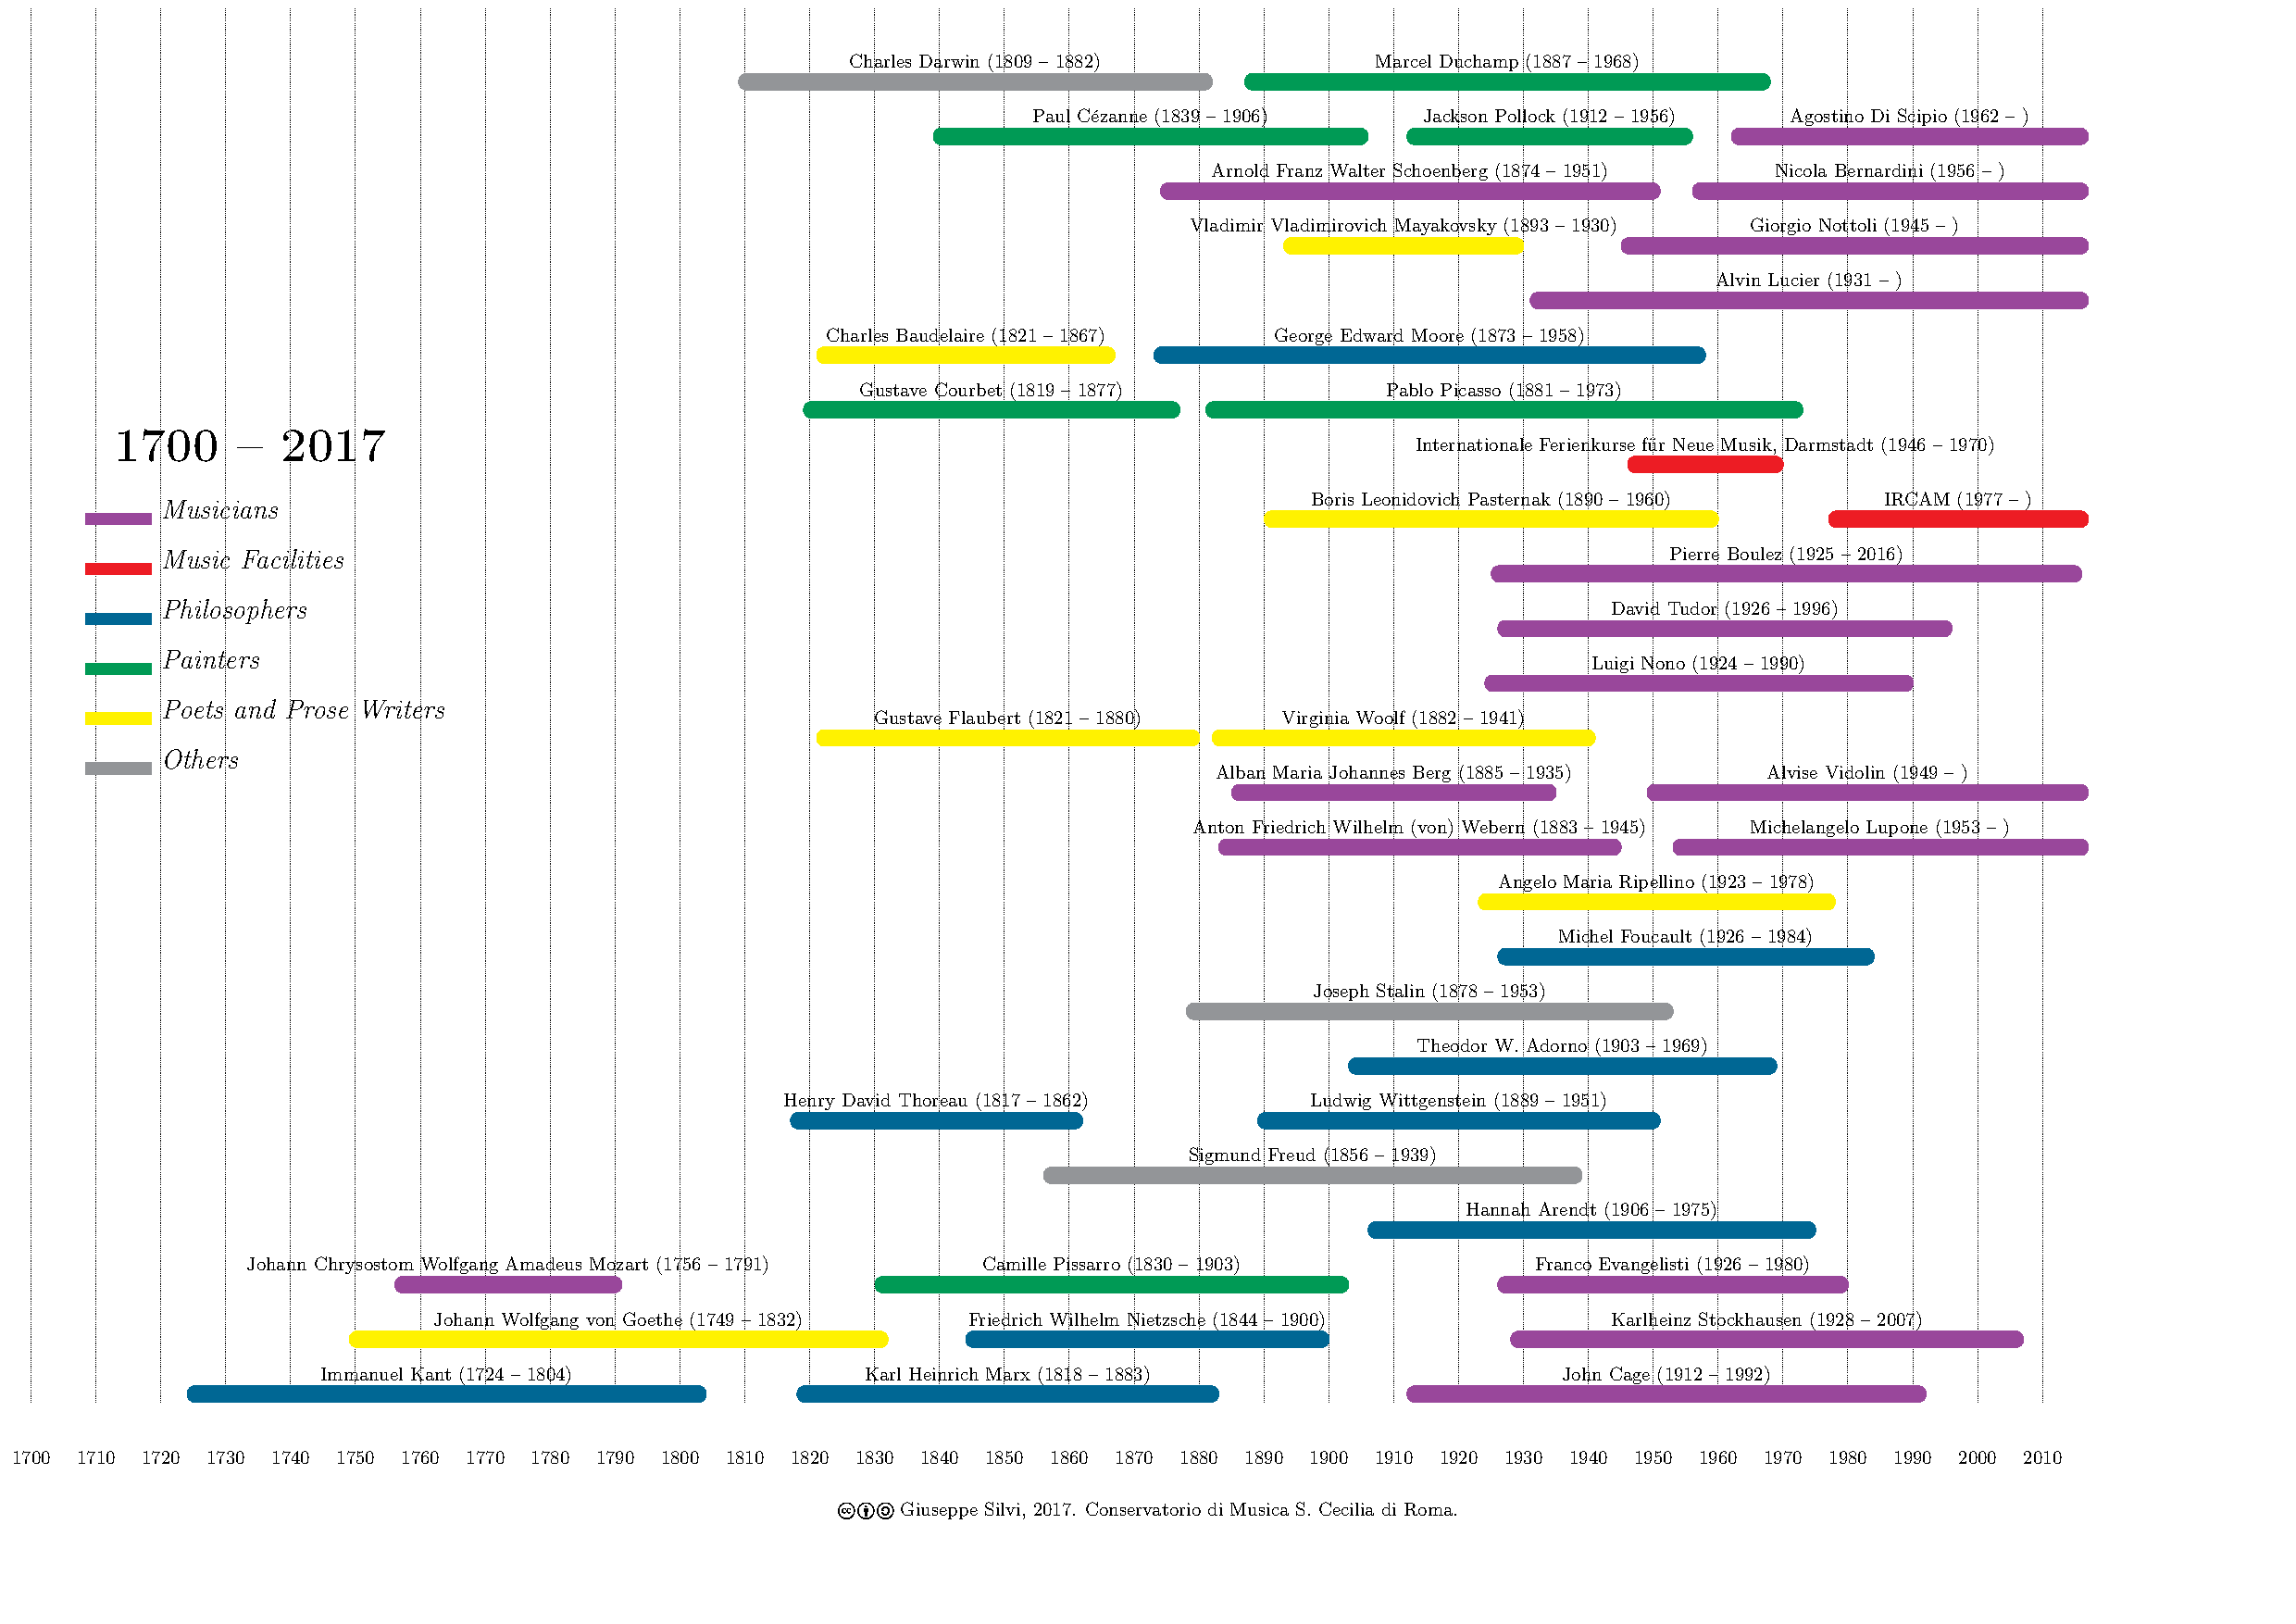
\includepdf[scale=2.0, offset= -430 0]{includes/_timeline/cosmologia.pdf}
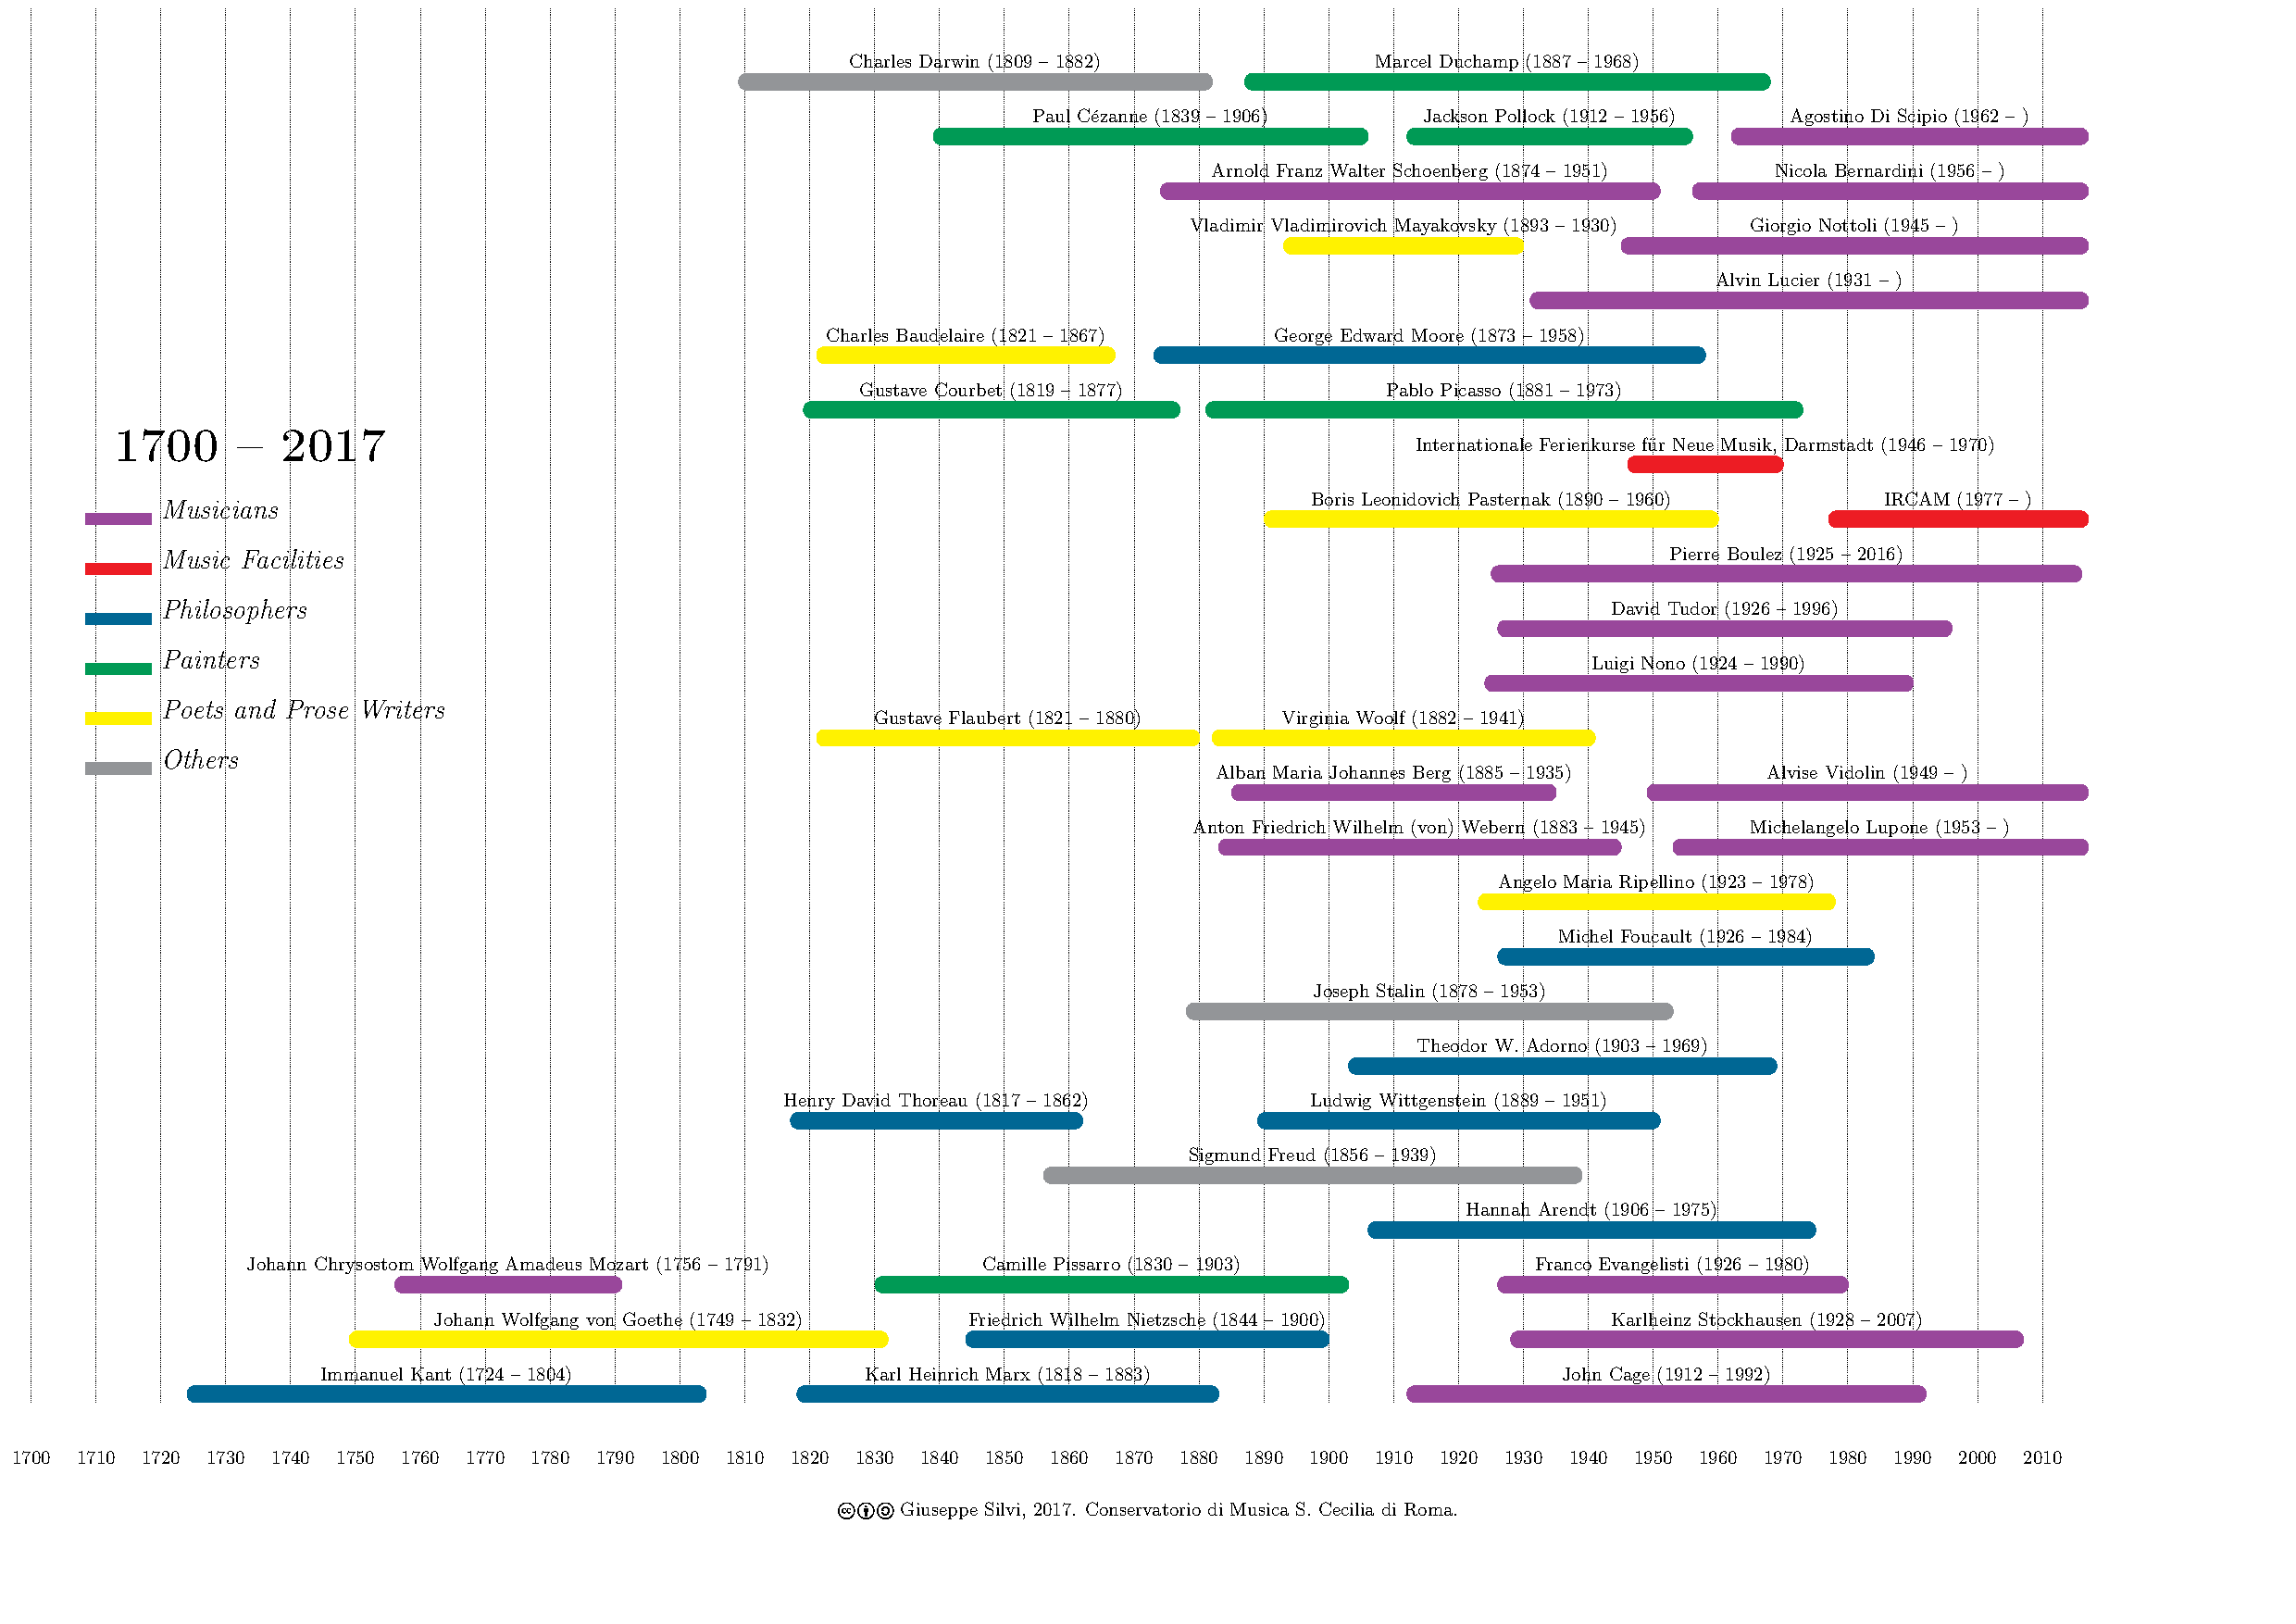
\includepdf[scale=2.0, offset= -410 0]{includes/_timeline/cosmologia.pdf}

\end{document}
